\documentclass[journal]{IEEEtran}
\usepackage{amsmath,amsfonts}
\usepackage{array}
\usepackage[caption=false,font=normalsize,labelfont=sf,textfont=sf]{subfig}
\usepackage{textcomp}
\usepackage{stfloats}
\usepackage{url}
\usepackage{verbatim}
\usepackage{graphicx}
\usepackage{cite}
\usepackage{hyperref}
\hypersetup{
	colorlinks=true,
	linkcolor=blue,   % 设置链接为蓝色
	citecolor=blue,
	urlcolor=blue,
}
\usepackage{tabularx}
\usepackage{threeparttable}
\usepackage{booktabs}
\usepackage{algpseudocode}
\usepackage{algorithm}

\hyphenation{op-tical net-works semi-conduc-tor IEEE-Xplore}
% updated with editorial comments 8/9/2021
\usepackage{xcolor}
\usepackage{siunitx}

\begin{document}

\title{Dynamic Path Gain Compensation for Enhancing Intracardiac Communication in Leadless Pacemakers}

\author{
  Dongming Li, \IEEEmembership{Student Member, IEEE},
 Zhijiong Wang, \IEEEmembership{Student Member, IEEE},
  Han Wang, \IEEEmembership{Student Member, IEEE},
  Sio Hang Pun, \IEEEmembership{Senior Member, IEEE},
  Peng Un Mak, \IEEEmembership{Senior Member, IEEE},
  Anguo Zhang, \IEEEmembership{Senior Member, IEEE},
  Yu Liu, \IEEEmembership{Member, IEEE},
  Hung-Chun Li,
  Yueming Gao, \IEEEmembership{Senior Member, IEEE},
  Min Du and Mang I Vai, \IEEEmembership{Senior Member, IEEE}
% --- Your author info and thanks can be placed here ---
}

\maketitle

\begin{abstract}
Implantable Medical Devices (IMDs) are evolving from isolated units into collaborative in-body networks, a paradigm shift whose central challenge is achieving reliable, ultra-low-power wireless communication within dynamic and pathological biological environments. Among all scenarios, multi-chamber leadless cardiac pacemaker (LCP) systems present the ultimate test for communication robustness, as they operate within the heart—the body's most mechanically active and pathologically complex organ. This paper directly confronts this challenge by proposing an adaptive receiver architecture with a universally applicable design philosophy. At its core is a hybrid analog-digital Automatic Gain Control (AGC) system, deeply co-designed with a power-efficient Super-Regenerative Receiver (SRR), to actively compensate for the severe, irregular channel fluctuations induced by pathological rhythms characterized by intermittent conduction failure, such as Atrioventricular (AV) block. To rigorously validate this architecture's performance, we designed and implemented an \textit{ex-vivo} porcine heart platform capable of precisely emulating such representative pathological dynamics. Experimental results on this platform show that the AGC successfully stabilizes the SRR input signal to within 1\% of its target level, even amidst channel gain variations exceeding 15\,dB. This stability translates into a dramatic improvement in communication reliability, with the Bit Error Rate (BER) reduced by up to 83.7\% at a 5\,kbps data rate. This work not only provides a key enabling technology for LCPs but, more importantly, offers a robust design paradigm and a rigorously validated solution for the next generation of networked IMDs designed to operate in harsh biological environments.
\end{abstract}

\begin{IEEEkeywords}
Leadless Pacemakers (LCPs), Galvanic Conductive Communication (GCC), Automatic Gain Control (AGC), Super-regenerative Receiver (SRR), Pathological Channel Dynamics, Atrioventricular Block.
\end{IEEEkeywords}


\section{Introduction}
\label{sec:introduction}

\IEEEPARstart{I}{mplantable} Medical Devices (IMDs) are undergoing a paradigm shift from isolated, standalone units to distributed, networked systems~\cite{Ferguson2011WirelessCW,zrenner2002will,laizou1999signal,Germanovix2000DesignOA}. The future of advanced healthcare will rely on deploying multiple miniature, intelligent sensing, monitoring, or therapeutic nodes within the human body, forming cooperative ``In-Body Networks"~\cite{estudillo2010intrabody,warren2010wireless,lin2014design}. To realize this vision, a central technological bottleneck must be overcome: establishing a long-term, stable, and ultra-low-power wireless communication link within the complex and perpetually dynamic biological environment.

To enable cooperation among multi-node IMDs, academia has explored various wireless technologies. However, conventional radio-frequency (RF) communication faces severe signal attenuation within the human body, typically necessitating high power consumption to maintain a link~\cite{bose2018rf}. While magnetic inductive coupling offers lower power, it is constrained by its short communication range and stringent alignment requirements~\cite{li2018200mb}. Ultrasonic communication, in turn, is hampered by its inherent directionality, making it unreliable for non-line-of-sight scenarios~\cite{seyedi2013survey}. These intrinsic limitations severely curtail their suitability for the next generation of networked IMDs, which demand miniaturization and ultra-low-power operation. In this context, Galvanic Conductive Communication (GCC) emerges as a promising and potentially disruptive technology. GCC cleverly utilizes human tissue itself as the transmission medium, propagating information via a faint electric field. This approach not only offers the potential for extremely low power consumption and simpler circuit implementation but also provides enhanced security, as the signal is naturally confined within the body. Given these distinct advantages, GCC has become one of the most promising candidates for enabling next-generation networked IMDs~\cite{wu2020equivalent, opie2004heart, Wegmueller2010Signal, 2016Galvanically}.

Among all implantable communication scenarios, the multi-chamber Leadless Cardiac Pacemaker (LCP) system represents the ultimate ``proving ground" for the robustness of GCC technology~\cite{middour2021leadless, malaczynska2023leadless,li2025dynamic}. Consequently, extensive research has been dedicated to characterizing the Intracardiac Communication (CIC) channel. Early investigations predominantly relied on static or quasi-static models, employing finite element analysis, numerical simulations, and \textit{in-vivo} animal studies to delineate fundamental transmission properties~\cite{bereuter2018fundamental, wang2024analysis,khaleghi2020conductive, maldari2020wide}. More recently, as research has matured, the dynamic nature of the CIC has gained attention. For instance, the work of \cite{chen2022investigation} provided valuable experimental insights into normal cardiac cycle dynamics via an \textit{ex-vivo} platform, while our group's prior work established a time-varying equivalent circuit model for such dynamic channels~\cite{wei2024time}.

\begin{figure}[htbp]
    \centering
    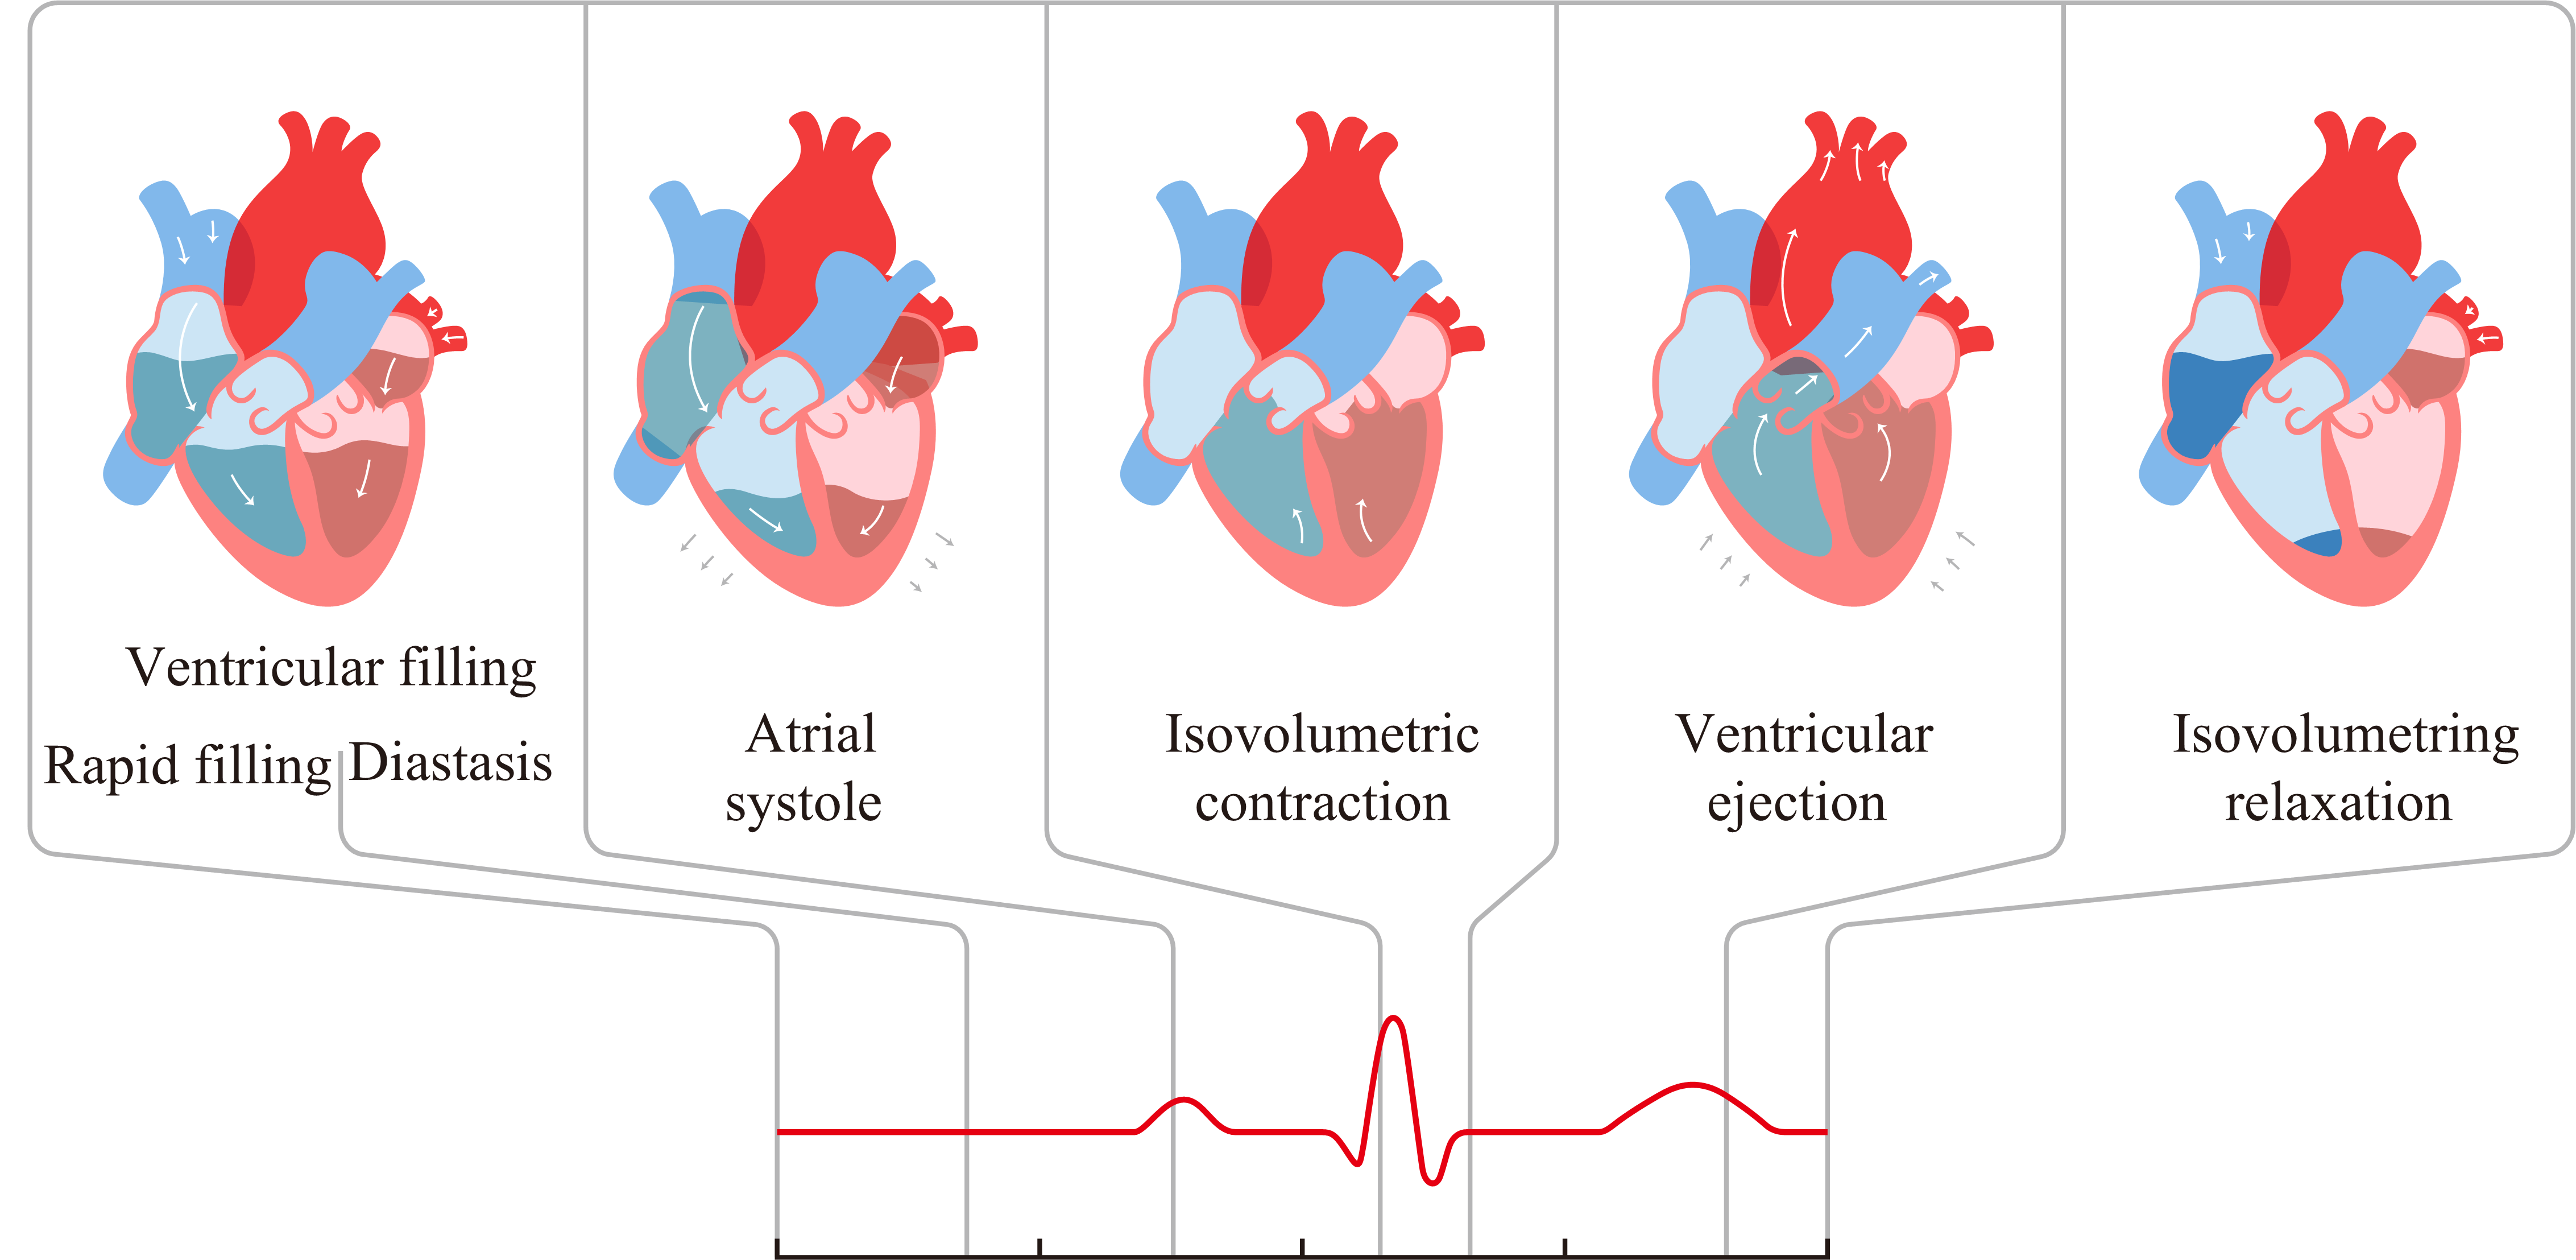
\includegraphics[width=8.5cm]{Figure/cycle}
    \caption{Illustration of the cardiac cycle, correlating the key electrical events of the electrocardiogram (ECG) with their corresponding mechanical phases, such as atrial systole and ventricular ejection.}
    \label{fig:1}
\end{figure}

These foundational studies are indispensable first steps. However, a critical challenge emerges as research transitions from theoretical feasibility to clinical robustness. Many existing CIC transceiver designs, in their early stages, inevitably rely on static or averaged channel models~\cite{ryser2022modulation,bereuter2019leadless,khaleghi2020conductive}. This idealized approximation, while convenient for initial analysis, masks a crucial fact: the intracardiac channel dynamics exist on two distinct levels. The first level is the ``healthy dynamic." As illustrated in Fig.~\ref{fig:1}, the regular heartbeat, even under normal sinus rhythm, induces predictable, periodic fluctuations in channel gain due to myocardial and hemodynamic shifts. However, the second, more severe level—and one that has been systematically overlooked—is the ``pathological dynamic." The channel environment induced by clinical conditions characterized by intermittent conduction failure is far from benign. A representative form of such a condition, an Atrioventricular (AV) block, is shown in Fig.~\ref{fig:0}; it exhibits chaotic, drastic, and highly unpredictable fluctuations. The vast majority of existing transceivers, lacking targeted consideration for these harsh ``pathological dynamics," harbor a significant vulnerability when faced with real-world clinical challenges, forming a fundamental barrier to translating prototypes into clinically reliable devices.

The choice of receiver architecture becomes paramount in addressing this ultimate challenge. Given the extremely stringent constraints on power and complexity in LCPs, the Super-Regenerative Receiver (SRR) architecture emerges as one of the most promising candidates, by virtue of its inherent simplicity and immense potential for achieving high sensitivity at very low power~\cite{frey2013improved,macfarlane1948theory}. The SRR architecture, however, is a double-edged sword: its performance exhibits extreme sensitivity to variations in the input signal amplitude~\cite{chen2007fully,vidojkovic20112}. While this characteristic can be exploited for high gain under stable channel conditions, it transforms into a critical liability in the dynamic CIC environment we face, necessitating a sophisticated compensatory mechanism to unlock the SRR's full potential.

Therefore, Automatic Gain Control (AGC) is an indispensable component for ensuring system robustness. Yet, conventional AGC solutions are not directly applicable to LCPs. Fully analog AGC systems, while offering rapid response, often suffer from poor linearity, imprecise gain control, and a fixed-threshold operation that limits adaptability in complex, varying environments~\cite{Zhao2023AnAF}. Conversely, fully digital AGC solutions, while capable of high precision and flexibility, come at the cost of significant computational overhead and power consumption, which is incompatible with the microwatt-level budget of an LCP~\cite{Li2020DigitalAC}. Consequently, there is a pressing technological need for an AGC solution that optimally synergizes rapid response, precise control, and extreme power efficiency.

In response to this imperative, this paper introduces a novel SRR system integrated with a meticulously co-designed hybrid analog-digital AGC mechanism. This architecture strategically leverages the rapid response of an analog front-end with the intelligent, fine-grained control afforded by digital processing, aiming to achieve robust compensation for dynamic CIC path gain variations while rigorously adhering to LCP power constraints. The main contributions of this work can be summarized as follows:

\begin{itemize}
    \item We propose a novel hybrid AGC receiver architecture, co-designed with an SRR, whose design principles can be extended to other IMDs operating in dynamic biological environments.
    \item We designed and implemented an \textit{ex-vivo} experimental platform capable of accurately emulating the dynamics of a representative pathological arrhythmia, providing a controllable and repeatable methodology for investigating communication challenges in harsh biological environments.
    \item For the first time, we systematically incorporate the complex channel dynamics induced by this representative clinical pathology into the entire design, optimization, and validation workflow of a transceiver, bridging a critical gap between existing research and clinical reality.
    \item This research provides a valuable theoretical basis and a practical example for designing adaptive transceivers that can operate robustly in volatile biological environments, paving the way for the development of next-generation, high-performance, and high-reliability networked IMDs.
\end{itemize}

\begin{figure}[htbp]
    \centering
    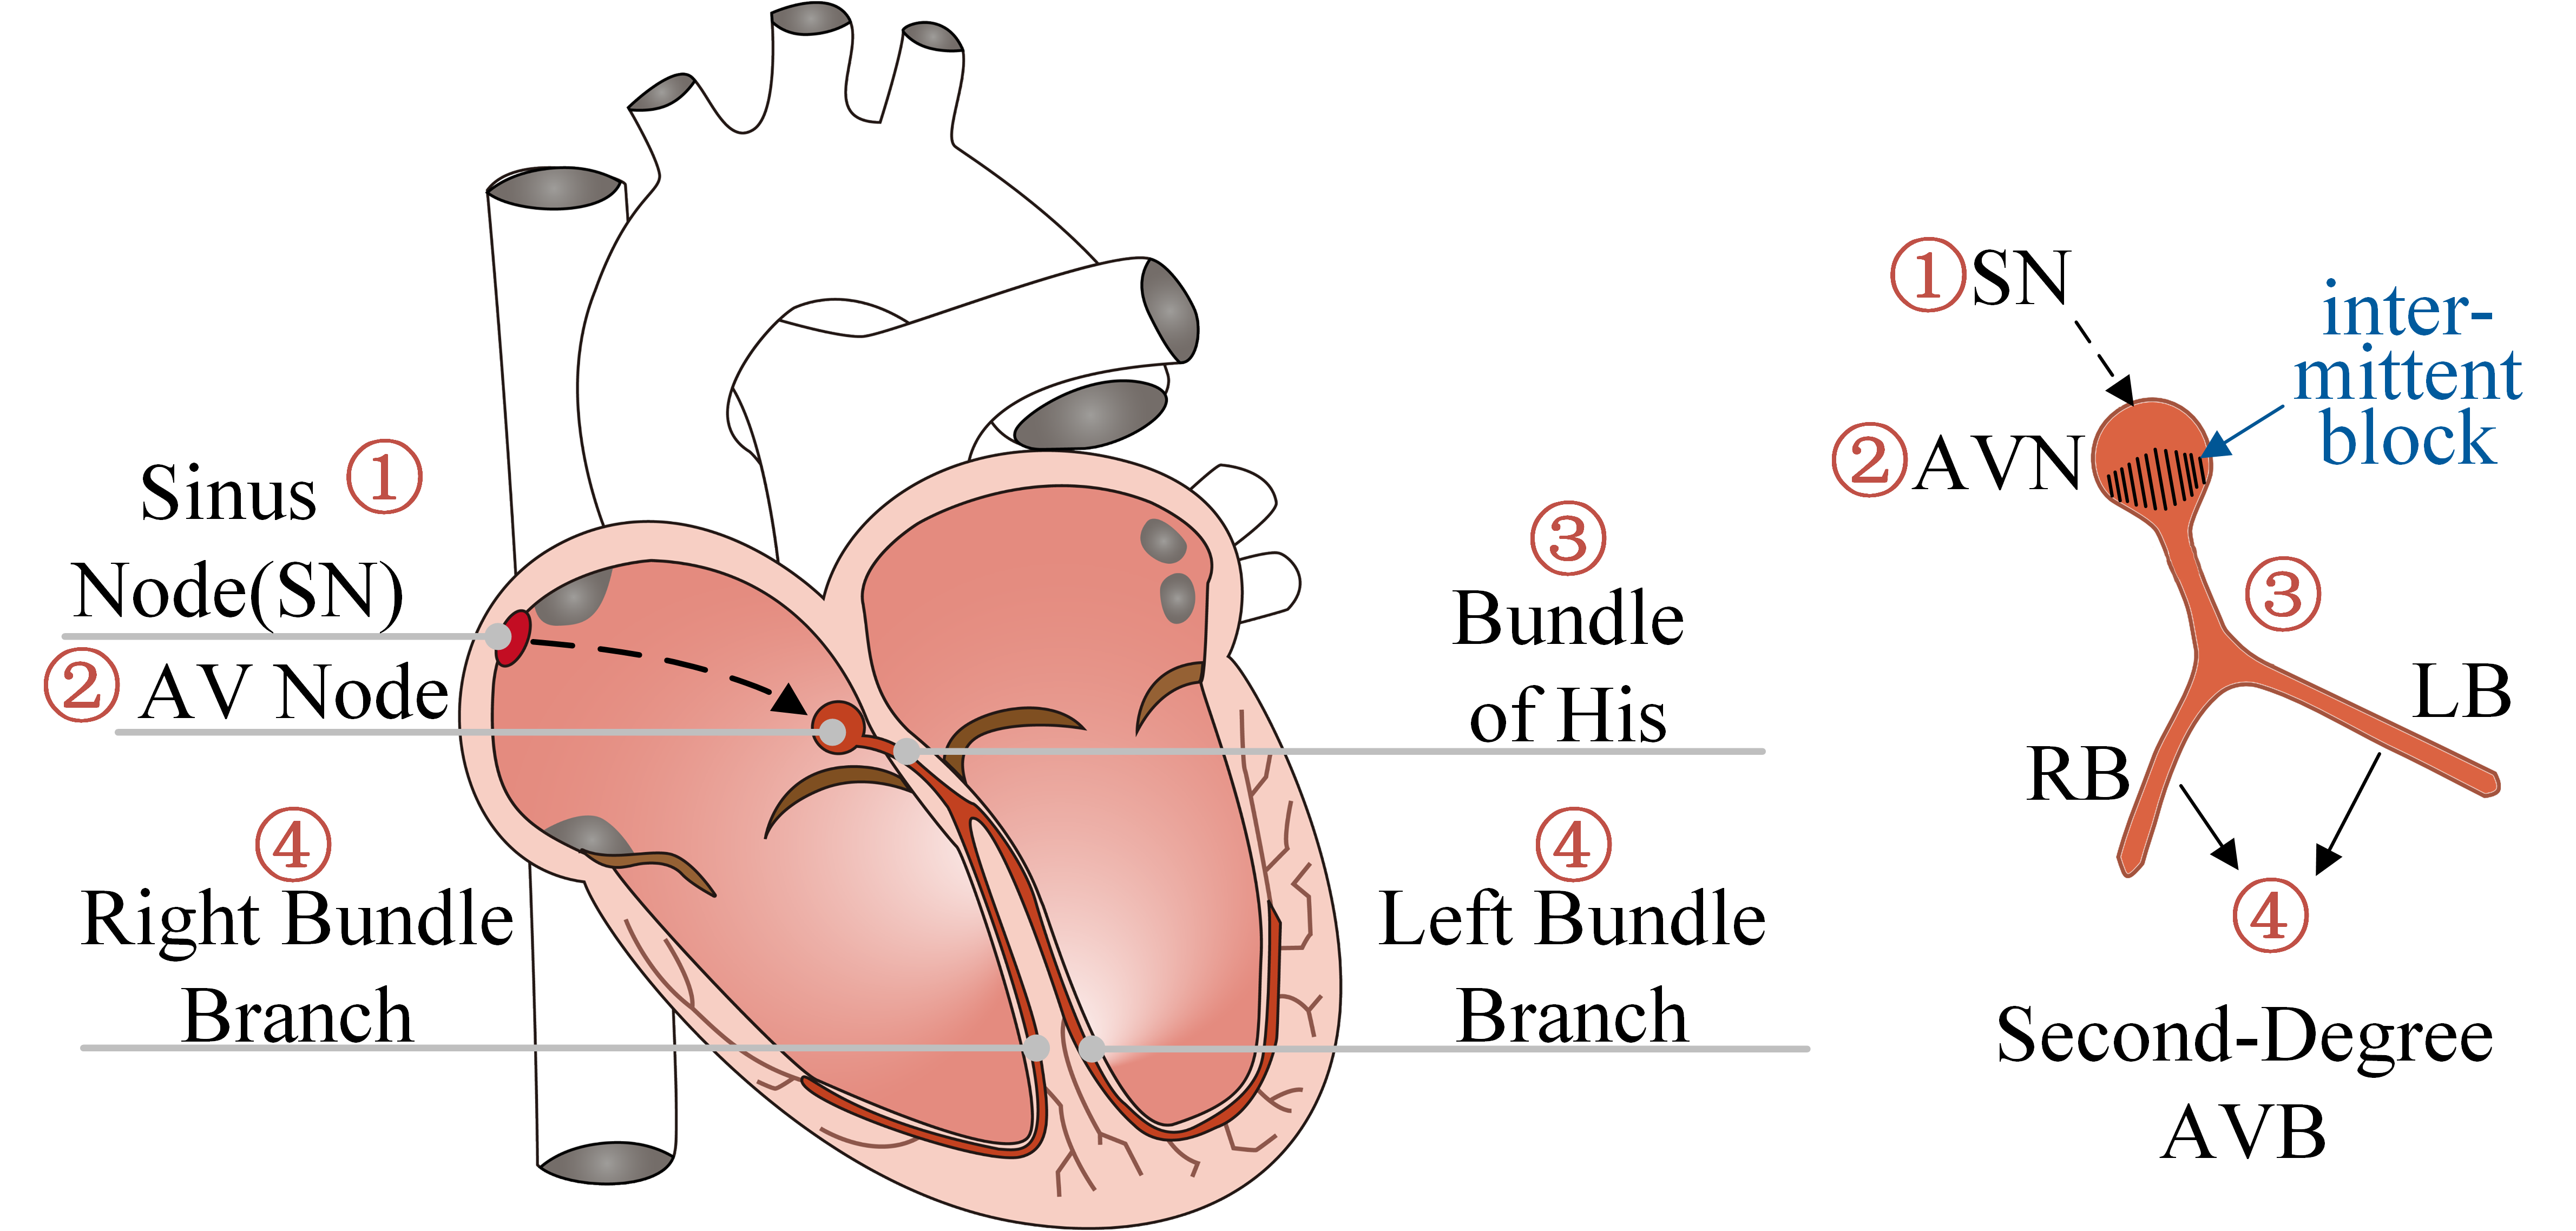
\includegraphics[width=8.3cm]{Figure/AVB}
    \caption{Schematic diagram of the cardiac conduction system and a representative Atrioventricular Block (Second-degree Type I).}
    \label{fig:0}
\end{figure}

\section{Methods}\label{sec:Methods}
\subsection{Dynamic Channel Characteristics and Impact on Receiver Performance}
\label{subsec:channel_and_impact}

Effective intra-cardiac communication for multi-chamber leadless pacemakers is fundamentally constrained by the dynamic physiological environment. The rhythmic electromechanical activity of the heart induces profound temporal variations in the CIC channel gain, denoted as~$G_c(t)$~\cite{wei2024time}. This challenge is profoundly exacerbated under the very pathological conditions, such as arrhythmogenic profiles, that necessitate pacing. These conditions engender channel fluctuations that are far more complex, erratic, and severe than those observed during normal sinus rhythm. Maintaining reliable communication amidst such volatility constitutes a formidable and central challenge, which this work aims to address.

While the SRR architecture is an attractive candidate due to its high sensitivity and low power consumption, its performance is acutely dependent on the stability of its input signal amplitude,~$A_{in}(t)$. This sensitivity is an intrinsic consequence of its operating principle. A simplified equivalent parallel resonant circuit model of the SRR is shown in Fig.~\ref{fig:srr_model}.

\begin{figure}[h]
    \centering
    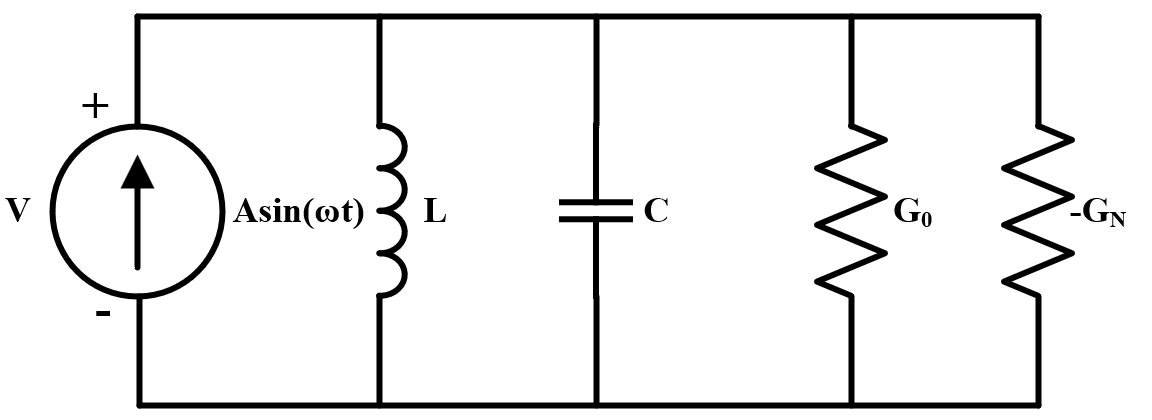
\includegraphics[width=0.7\columnwidth]{Figure/model}
    \caption{Equivalent parallel resonant circuit model of a super-regenerative oscillator, where the total conductance is~$G = G_o - G_N$.}
    \label{fig:srr_model}
\end{figure}

The core principle is predicated on periodically switching the oscillator's total parallel conductance,~$G$, between a negative value (the regeneration phase) and a positive value (the quenching phase). During regeneration, a negative conductance,~$-G_N$, provided by the active device, overcomes the tank's inherent losses,~$G_o$, yielding a net negative conductance~($G = G_o - G_N < 0$). This condition establishes an unstable positive feedback loop, wherein the tank voltage,~$V(t)$, grows exponentially from any initial perturbation. The voltage envelope,~$V_{env}(t)$, follows the relation:
\begin{equation}
    V_{env}(t) \propto e^{-\alpha t}, \quad \text{where} \quad \alpha = \frac{G}{2C}
    \label{eq:srr_growth}
\end{equation}
Since~$G < 0$ during regeneration, the damping factor~$\alpha$ is negative, resulting in exponential growth of the form~$e^{|\alpha|t}$. The input signal,~$A_{in}(t)$, serves as the initial ``seed" for this exponential growth. Consequently, a stronger input signal yields a significantly larger final envelope amplitude over a fixed regeneration period.

In a front-end without adaptive control, the SRR's input amplitude,~$A_{in}(t)$, is directly modulated by the volatile channel gain:
\begin{equation}
    A_{in}(t) = G_{LNA} \cdot G_c(t) \cdot A_{tx}
    \label{eq:ain_channel}
\end{equation}
where~$G_{LNA}$~is the gain of the preceding Low Noise Amplifier (LNA) and~$A_{tx}$~is the transmitted signal amplitude. As a direct consequence,~$A_{in}(t)$~experiences substantial variations synchronous with the cardiac cycle.

Since the SRR's output envelope is directly proportional to its input amplitude, $A_{in}(t)$, and signal power is proportional to the square of the amplitude, this input instability leads to a severe degradation in demodulation performance. The effective signal-to-noise ratio at the SRR's decision point, $SNR_{eff}(t)$, exhibits a quadratic dependence on the input signal amplitude:
\begin{equation}
    SNR_{eff}(t) = \kappa \frac{A_{in}(t)^2}{N_{eff}}
    \label{eq:snr_squared}
\end{equation}
where~$\kappa$~is a proportionality constant and~$N_{eff}$~is the equivalent input noise level. This quadratic relationship means that even moderate fluctuations in~$A_{in}(t)$~are magnified into severe variations in~$SNR_{eff}(t)$.

This cascade of dependencies results in a catastrophic decline in communication reliability. For On-Off Keying (OOK) modulation in an Additive White Gaussian Noise (AWGN) channel, the instantaneous bit error probability,~$P_e(t)$, is dictated by the complementary error function (erfc) of the instantaneous SNR:
\begin{equation}
    P_e(t) = \frac{1}{2}\text{erfc}\left(\sqrt{\frac{SNR_{eff}(t)}{2}}\right)
    \label{eq:Pe_t_revised}
\end{equation}
The overall, long-term Bit Error Rate (BER), being the time-averaged integral of~$P_e(t)$, has severe implications. During deep channel fades, the collapse of~$G_c(t)$~and consequently~$SNR_{eff}(t)$~causes~$P_e(t)$~to approach 0.5, signifying a momentary but complete link failure. Compounding this issue, the unstable input amplitude renders any fixed decision threshold,~$V_{th}$, inherently suboptimal, as the internal signal features leveraged for demodulation become highly variable. The confluence of these two critical issues---precipitous SNR degradation and the inherent suboptimality of a fixed decision threshold---provides the fundamental rationale for designing the adaptive compensation architecture that forms the basis of this work.

\subsection{Adaptive Receiver Architecture with Hybrid Gain Control}
\label{subsec:adaptive_architecture}
To counteract the severe performance degradation caused by dynamic channel fluctuations, we propose an adaptive receiver architecture incorporating a hybrid analog-digital AGC loop. This approach is designed to stabilize the signal amplitude at the input of the SRR core, thereby ensuring robust demodulation under any channel condition. Fig.~\ref{fig:framework} depicts a schematic of this architecture, which is a closed-loop feedback system engineered for the stringent power and complexity constraints of LCPs.

A key innovation of this architecture is its strategic exploitation of the self-quenching SRR's intrinsic operating principle. The circuit schematic of the SRR core is shown in Fig. \ref{fig:sro_schematic}. Unlike externally-quenched SRRs, our design employs an oscillator where the quenching mechanism is integrated directly into its own biasing network. This is achieved via a low-pass filter in the emitter path; as the oscillation envelope grows, rectified current charges this network, shifting the transistor's DC operating point to a non-oscillating region and thus intrinsically quenching the cycle.

The crucial aspect for amplification is that the incoming RF signal modulates this DC bias point. A stronger input signal creates a more favorable initial condition, which accelerates the oscillation build-up and produces a significantly larger output envelope within a single quenching period. This inherent characteristic—where the SRR's output envelope serves as a high-gain, amplified representation of its input amplitude—is precisely what our architecture leverages.

Leveraging the SRR's acute sensitivity to input amplitude, we have designed the following closed-loop feedback process to precisely stabilize this signal. The incoming RF signal is first processed by the LNA and subsequently routed to a Variable Gain Amplifier (VGA), which serves as the primary gain control element. Its gain is dynamically modulated by an analog control voltage. After the VGA, a Received Signal Strength Indicator (RSSI) module measures the signal's amplitude and generates a proportional DC voltage. This voltage is then digitized by an Analog-to-Digital Converter (ADC), yielding a discrete-time representation of the signal level for the microcontroller (MCU). The MCU executes a Proportional-Integral-Derivative (PID) control algorithm based on the discrepancy between this feedback value and a programmable setpoint to dynamically update the VGA's control voltage. This architecture thus establishes a complete closed-loop control system, ensuring the amplitude of the signal presented to the SRR remains stable, irrespective of channel dynamics.

\begin{figure}[!t]
    \centering
    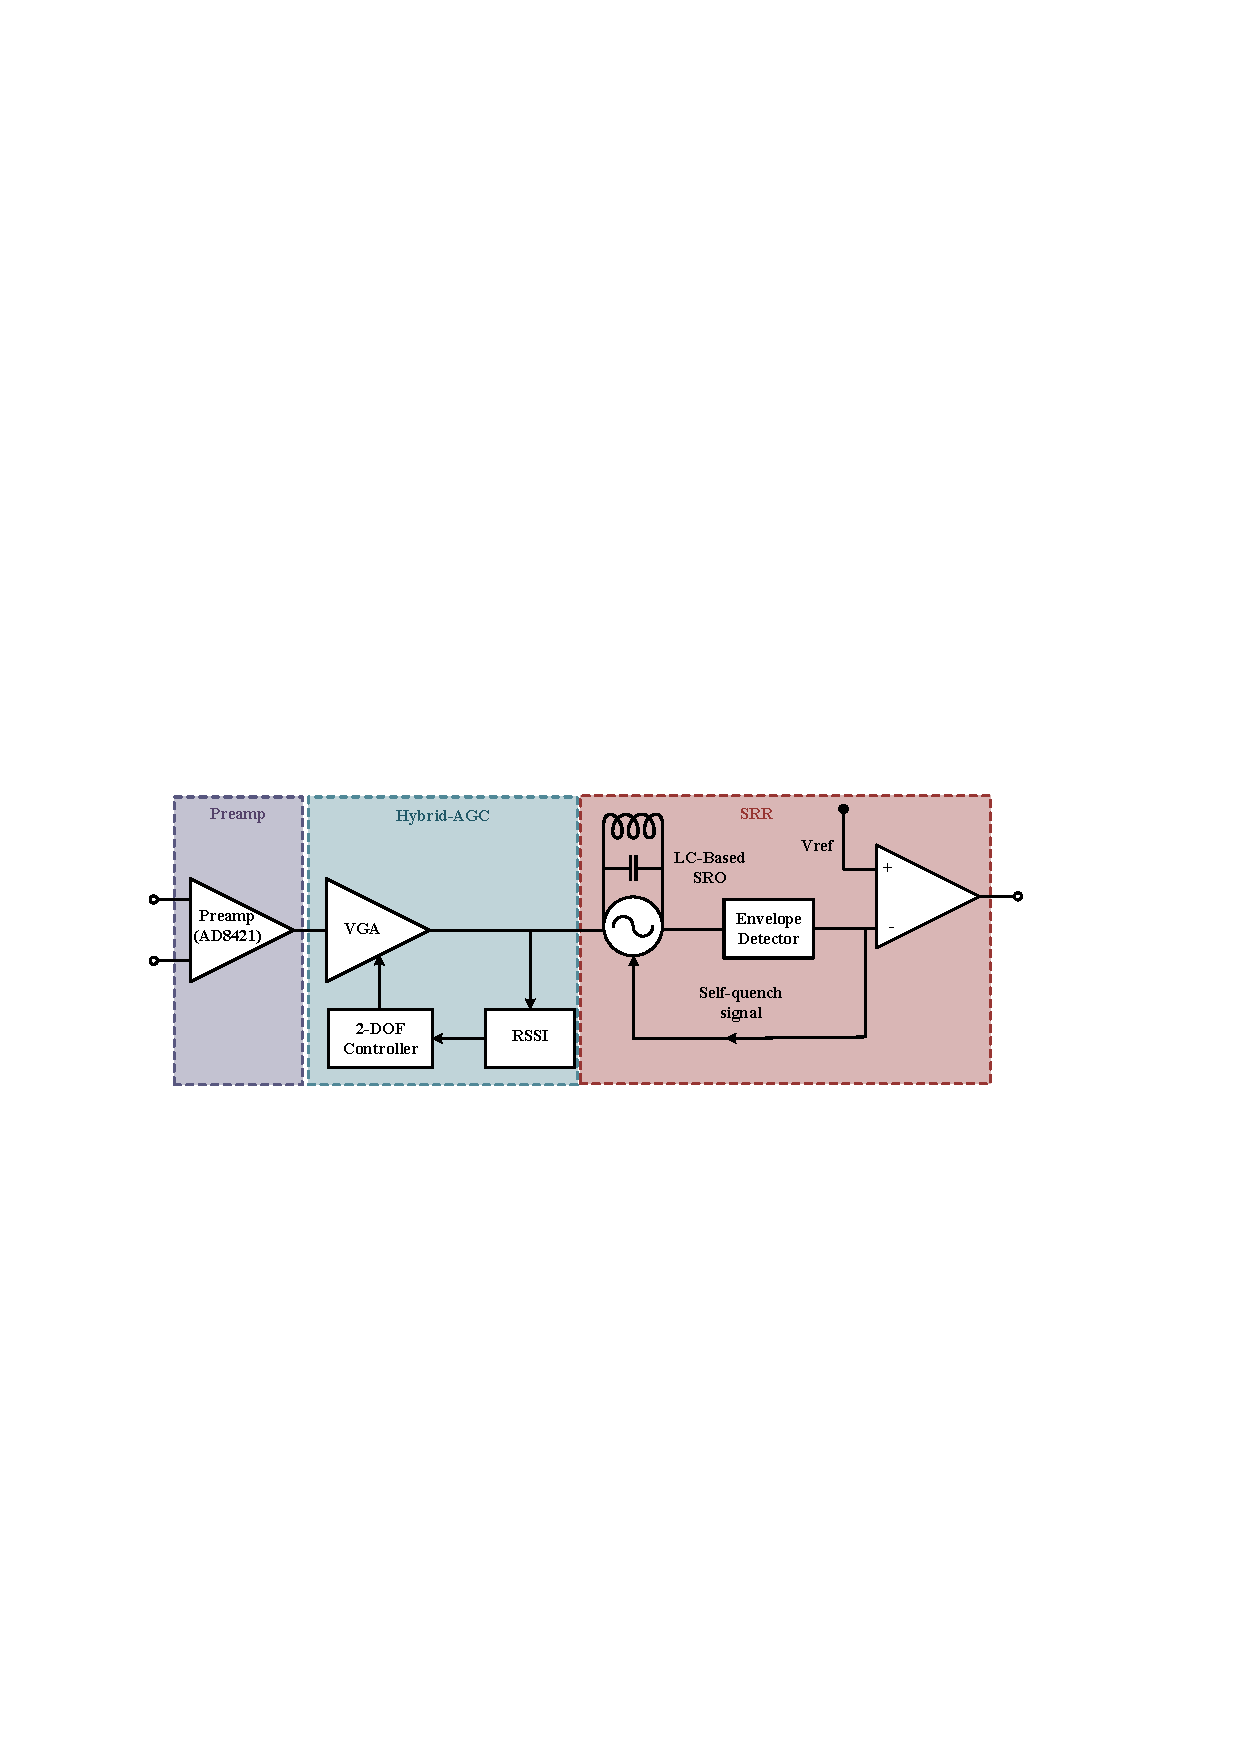
\includegraphics[width=8.3cm]{Figure/framework}
    \caption{Block diagram of the proposed adaptive receiver. The architecture comprises a preamplifier, a hybrid-AGC loop for signal stabilization, and an SRR core for demodulation. The SRR employs a self-quenching oscillator for power-efficient operation.}
    \label{fig:framework}
\end{figure}

\subsection{Gain Compensation Principle and PID Control Algorithm}
\label{subsec:principle_and_algorithm}
The fundamental principle of the proposed AGC system is to dynamically adjust the VGA gain, $G_{VGA}$, to counteract the channel gain variations, $G_c(t)$, thereby maintaining a constant signal amplitude, $V_{target}$, at the SRR input. When the AGC loop achieves a stable state, the required $G_{VGA}$ can be derived from the overall system gain expression, yielding:
\begin{equation}
    G_{VGA}(t) \approx \frac{V_{target}}{G_{LNA} \cdot G_c(t) \cdot A_{tx}}
    \label{eq:GVGA_compensation}
\end{equation}

Equation~\eqref{eq:GVGA_compensation} lucidly illustrates that the AGC system must modulate $G_{VGA}(t)$ to be approximately inversely proportional to the instantaneous channel gain. This self-regulating action is orchestrated by the PID controller. For robust implementation, an incremental PID formulation is employed, where the controller calculates the necessary control effort increment, $\Delta u_k$, at each time step~\cite{wang2022incremental}. This is derived from the standard discrete-time PID representation:
\begin{equation}
    \Delta u_k = K_p (e_k - e_{k-1}) + K_i T_s e_k + \frac{K_d}{T_s} (e_k - 2e_{k-1} + e_{k-2})
    \label{eq:PID_standard_discrete}
\end{equation}
where $K_p, K_i, K_d$ are the gains, and $T_s$ is the sampling period. For efficient computation, this equation is rearranged as:
\begin{equation}
    \Delta u_k = k_1 e_k - k_2 e_{k-1} + k_3 e_{k-2}
    \label{eq:PID_computational_form}
\end{equation}
where the coefficients $k_1, k_2, k_3$ are pre-calculated from the PID gains and $T_s$. The cumulative digital control output is then converted by the ADC. The detailed iterative process is presented in Algorithm~\ref{alg:pid_control}. The selection of the PID gains was performed through a systematic, empirical tuning process directly on the experimental platform to optimize the transient and steady-state response, ensuring good stability and compensation performance across all tested heart preparations.

The choice of a PID controller is a deliberate design decision. A simple P-controller would suffer from steady-state error, while a PI controller would struggle to react to the sharp, unpredictable channel changes characteristic of a 'dropped beat' in an AVB cycle. The derivative (D) term is therefore crucial; it provides an anticipatory response to rapid changes in the channel gain, minimizing transient errors during these abrupt hemodynamic shifts.

\begin{figure}[!t]
    \centering
    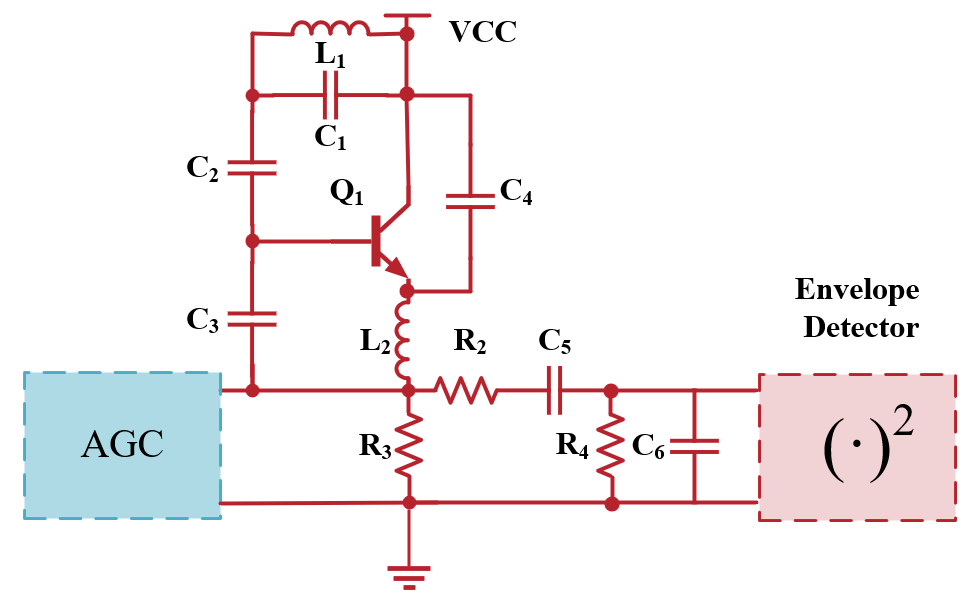
\includegraphics[width=0.75\columnwidth]{Figure/SRO}
    \caption{Circuit schematic of the self-quenching oscillator core. The self-quenching action is intrinsically governed by the transistor's biasing network.}
    \label{fig:sro_schematic}
\end{figure}

\begin{algorithm}[H]
    \caption{SRR Input Stabilization Algorithm}
    \label{alg:pid_control}
    \begin{algorithmic}[1] % [1] enables line numbering
        \Require
            $V_{\text{target,dig}}$, $k_1, k_2, k_3$, $u_{\text{min\_dig}}, u_{\text{max\_dig}}$
        \Ensure
            $V_c(k)$

        \State Initialize $u_{\text{prev}}$; $e_{\text{prev1}} \gets 0$; $e_{\text{prev2}} \gets 0$
        \While{system is operating}
            \State $A_{\text{in,detected}}(k) \gets \text{Sample And Digitize SRR Input}()$
            \State $e_k \gets V_{\text{target,dig}} - A_{\text{in,detected}}(k)$
            \State $\Delta u_k \gets k_1 e_k - k_2 e_{\text{prev1}} + k_3 e_{\text{prev2}}$
            \State $u_k \gets u_{\text{prev}} + \Delta u_k$
            \State $u_k \gets \text{saturate}(u_k, u_{\text{min\_dig}}, u_{\text{max\_dig}})$
            \State $V_c(k) \gets \text{Digital To Analog Conversion}(u_k)$
            \State $\text{Set VGA Control Voltage}(V_c(k))$
            \State \hspace{-1.5em} $\triangleright$ Update historical values for next iteration
            \State $e_{\text{prev2}} \gets e_{\text{prev1}}$
            \State $e_{\text{prev1}} \gets e_k$
            \State $u_{\text{prev}} \gets u_k$
        \EndWhile
    \end{algorithmic}
\end{algorithm}


\section{Experimental Methodology and Setup}
The efficacy of the proposed AGC system was rigorously validated through a comprehensive \textit{ex-vivo} experimental methodology.

\subsection{Dynamic Channel Emulation Platform and Characterization}
The cornerstone of the methodology was an \textit{ex-vivo} perfusion platform, depicted in Fig.~\ref{fig:agc_test_schematic}. The platform's biological core was a fresh porcine heart. Hemodynamic emulation was achieved via a dual-channel peristaltic pump system, which circulated a physiologically relevant simulated blood formulated to match the electrical conductivity of native human blood at 37°C~\cite{maldari2020wide, gabriel1996dielectric}. A host computer provided meticulous, time-varying control over intracardiac chamber volumes.

To validate our system under challenging pathological dynamics, we selected AVB—a condition characterized by intermittent conduction failure—as our model arrhythmia. Among the different types of AVB, Mobitz Type I presents an ideal and comprehensive test case for an adaptive system, as its characteristic Wenckebach phenomenon includes both progressive and abrupt changes. An adaptive system that can track this complex pattern demonstrates its capability to handle both gradual and sudden channel variations. Therefore, our platform was programmed to precisely replicate the hemodynamic profile of a Mobitz Type I AVB, serving as a representative model for a harsh pathological channel environment.

These profiles were carefully designed based on published human cardiac chamber volume data~\cite{maceira2010reference, 2006Normalized, 2006Reference, 2013Reference, chen2022investigation}. The resulting dynamic mappings for both Normal Sinus Rhythm (NSR) and our AVB model are illustrated in Fig.~\ref{fig:nsr_mapping} and Fig.~\ref{fig:avb_mapping}. The emulation was meticulously programmed; for instance, to accurately simulate the ``dropped beat'' characteristic, the control sequence included an atrial filling period that was not followed by a ventricular ejection. For initial characterization, a Vector Network Analyzer (VNA) was integrated with the platform to continuously measure the RA-RV channel's path gain.

\begin{figure}[!t]
    \centering
    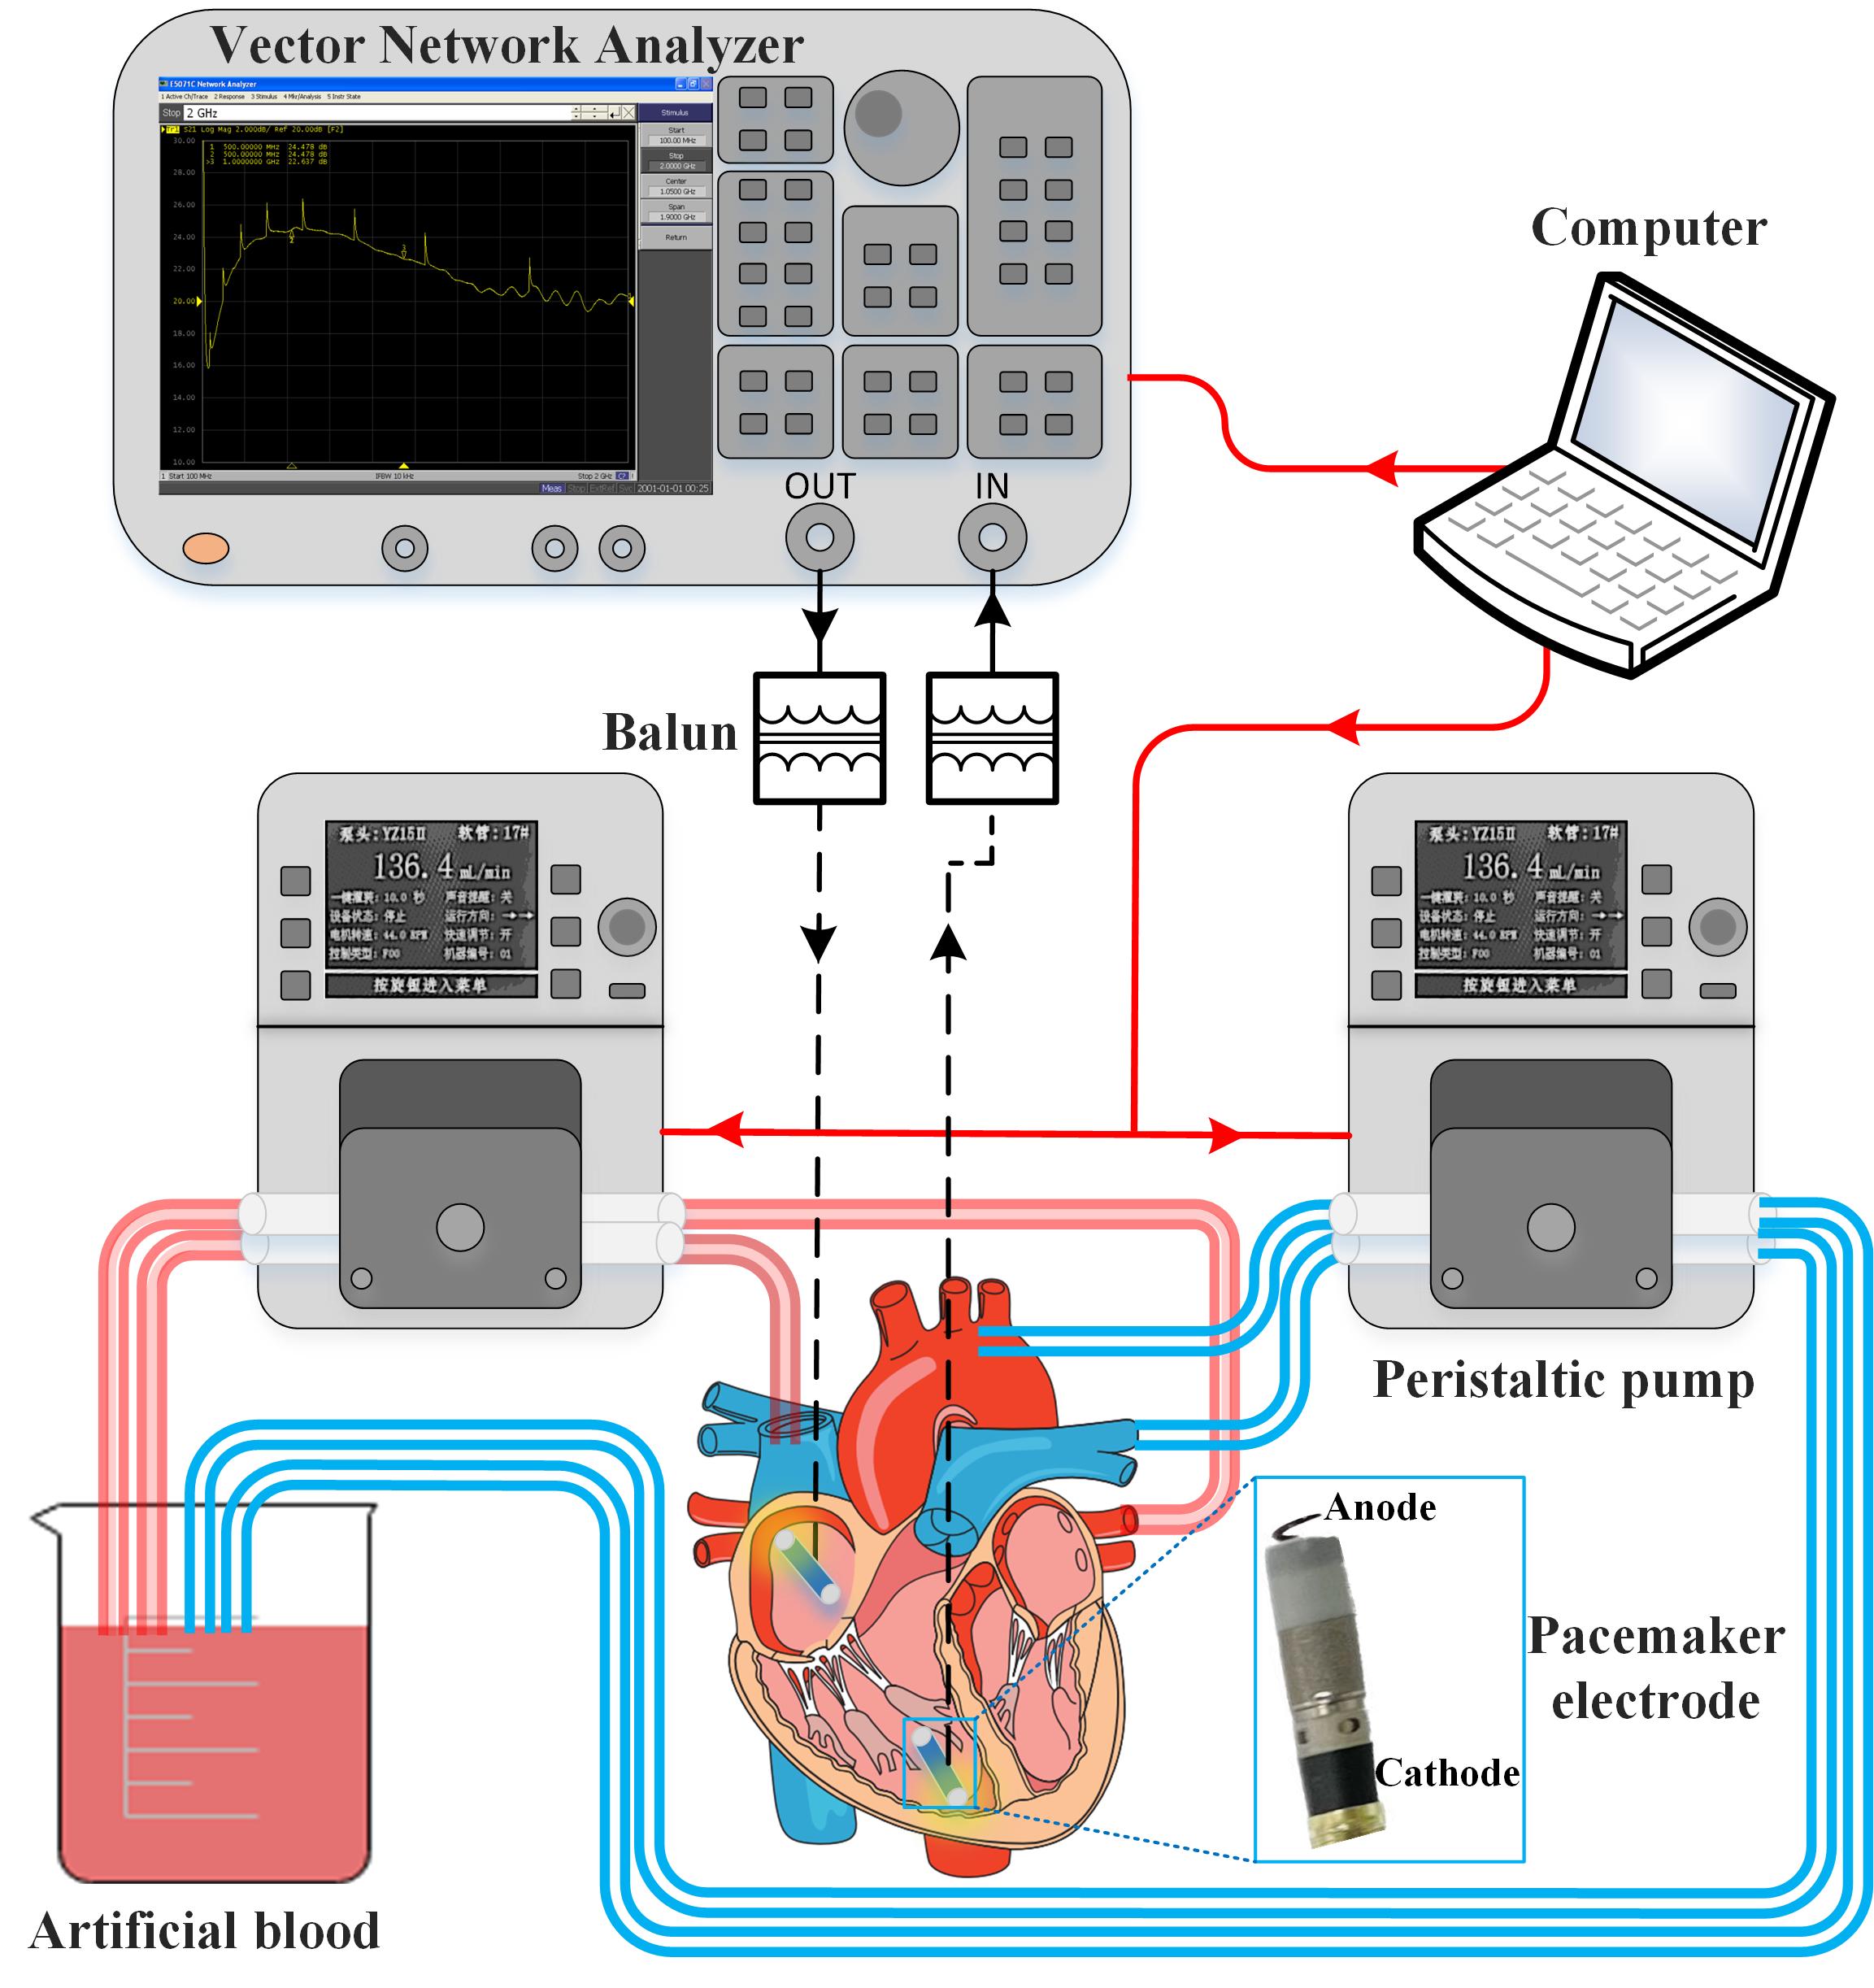
\includegraphics[width=0.9\columnwidth]{Figure/measure_setup.png}
    \caption{Photograph of the assembled experimental testbed, showcasing the peristaltic pump system, the cannulated \textit{ex-vivo} porcine heart, signal generation instrumentation, and the custom-developed receiver module. 1:1 baluns are used for galvanic isolation.}
    \label{fig:agc_test_schematic}
\end{figure}

\begin{table}[!t]
\centering
\caption{Cardiac Cycle Phases and Corresponding Chamber Volumes}
\begin{tabular}{cccc}
\hline
\text{\bfseries Phase} & \text{\bfseries Duration(s)} & \text{\begin{tabular}[c]{@{}c@{}}\bfseries Left Cardiac\\\bfseries Volume (mL)\end{tabular}} & \text{\begin{tabular}[c]{@{}c@{}}\bfseries Right Cardiac\\ \bfseries Volume (mL)\end{tabular}} \\ \hline
\text{Isovolumetric Relaxation} & 0.07 & 120.00 & 150.00 \\
\text{Rapid filling} & 0.11 & 173.44 & 202.88 \\
\text{Diastasis} & 0.22 & 191.25 & 220.50 \\
\text{Atrial Contraction} & 0.10 & 215.00 & 244.00 \\
\text{Isovolumetric Contraction} & 0.05 & 215.00 & 244.00 \\
\text{Rapid ejection} & 0.10 & 151.67 & 181.34 \\
\text{Slow ejection} & 0.15 & 120.00 & 150.00 \\ \hline
\end{tabular}
\label{tab:volume_data}
\end{table}

\begin{figure}[!t]
    \centering
    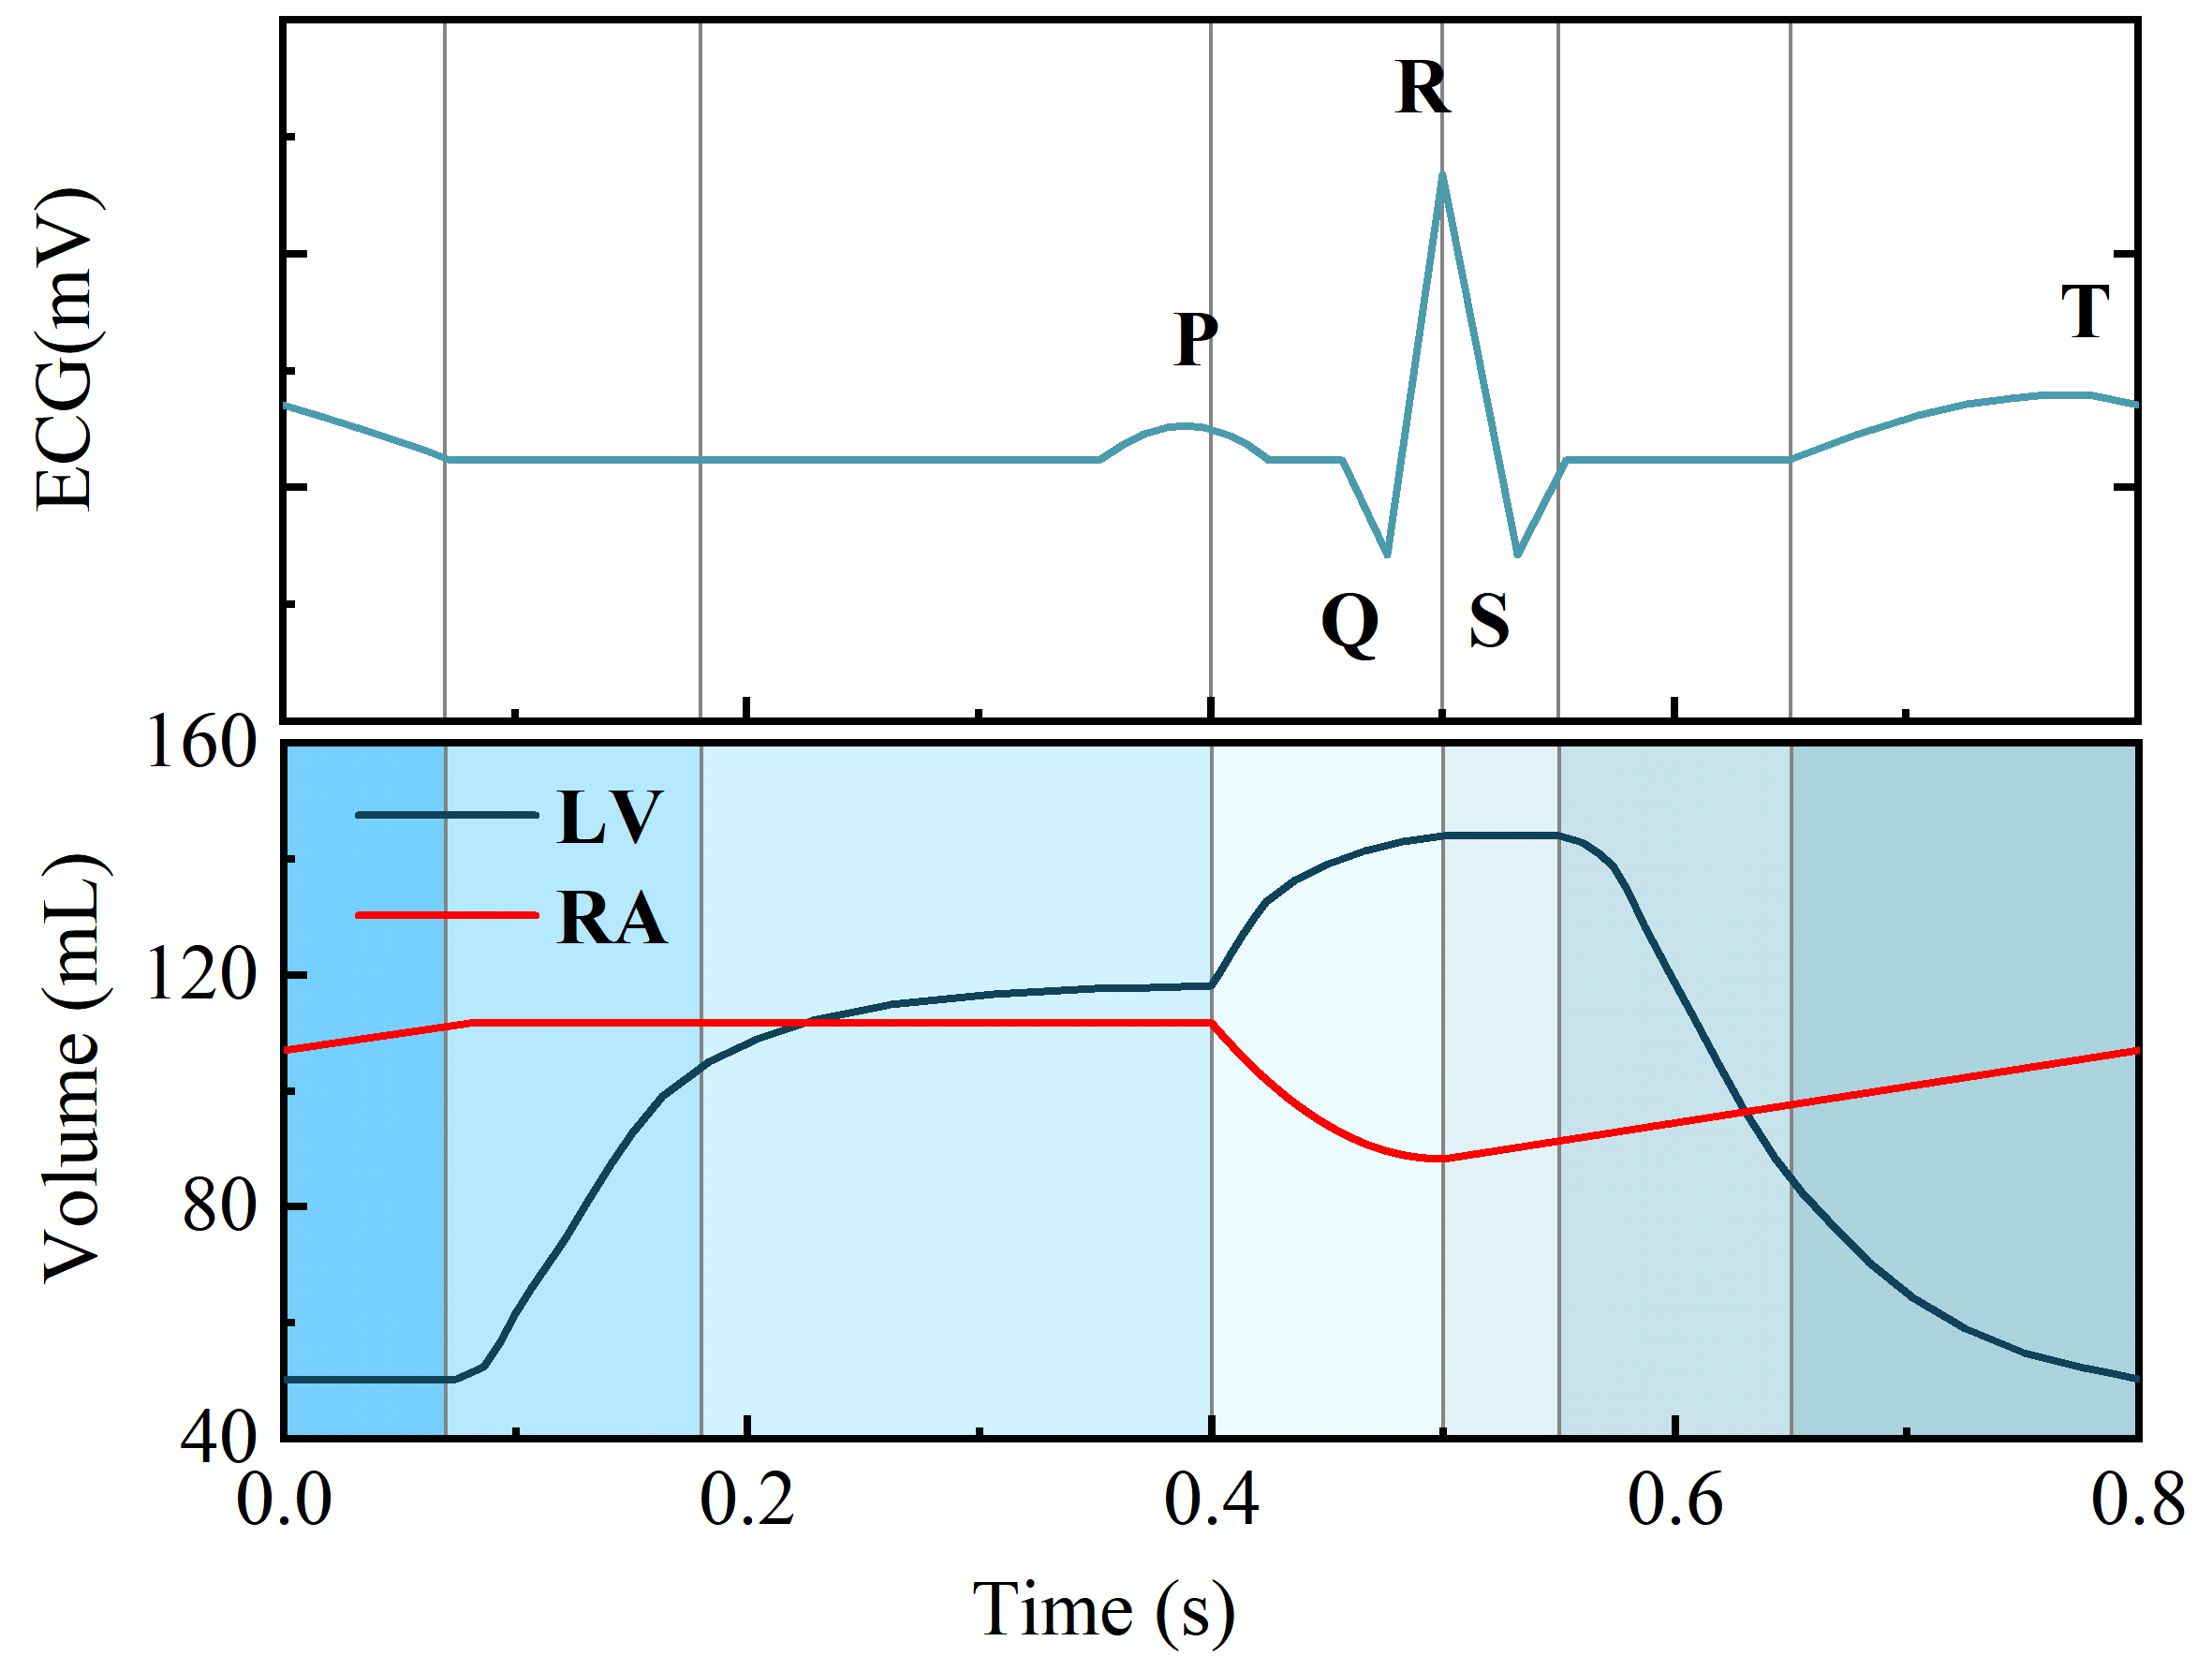
\includegraphics[width=0.9\columnwidth]{Figure/Nor_Vol}
    \caption{Dynamic mapping between the ECG and right-sided chamber volumes under simulated NSR. This served as the baseline model for a healthy heart.}
    \label{fig:nsr_mapping}
\end{figure}

\begin{figure}[!t]
    \centering
    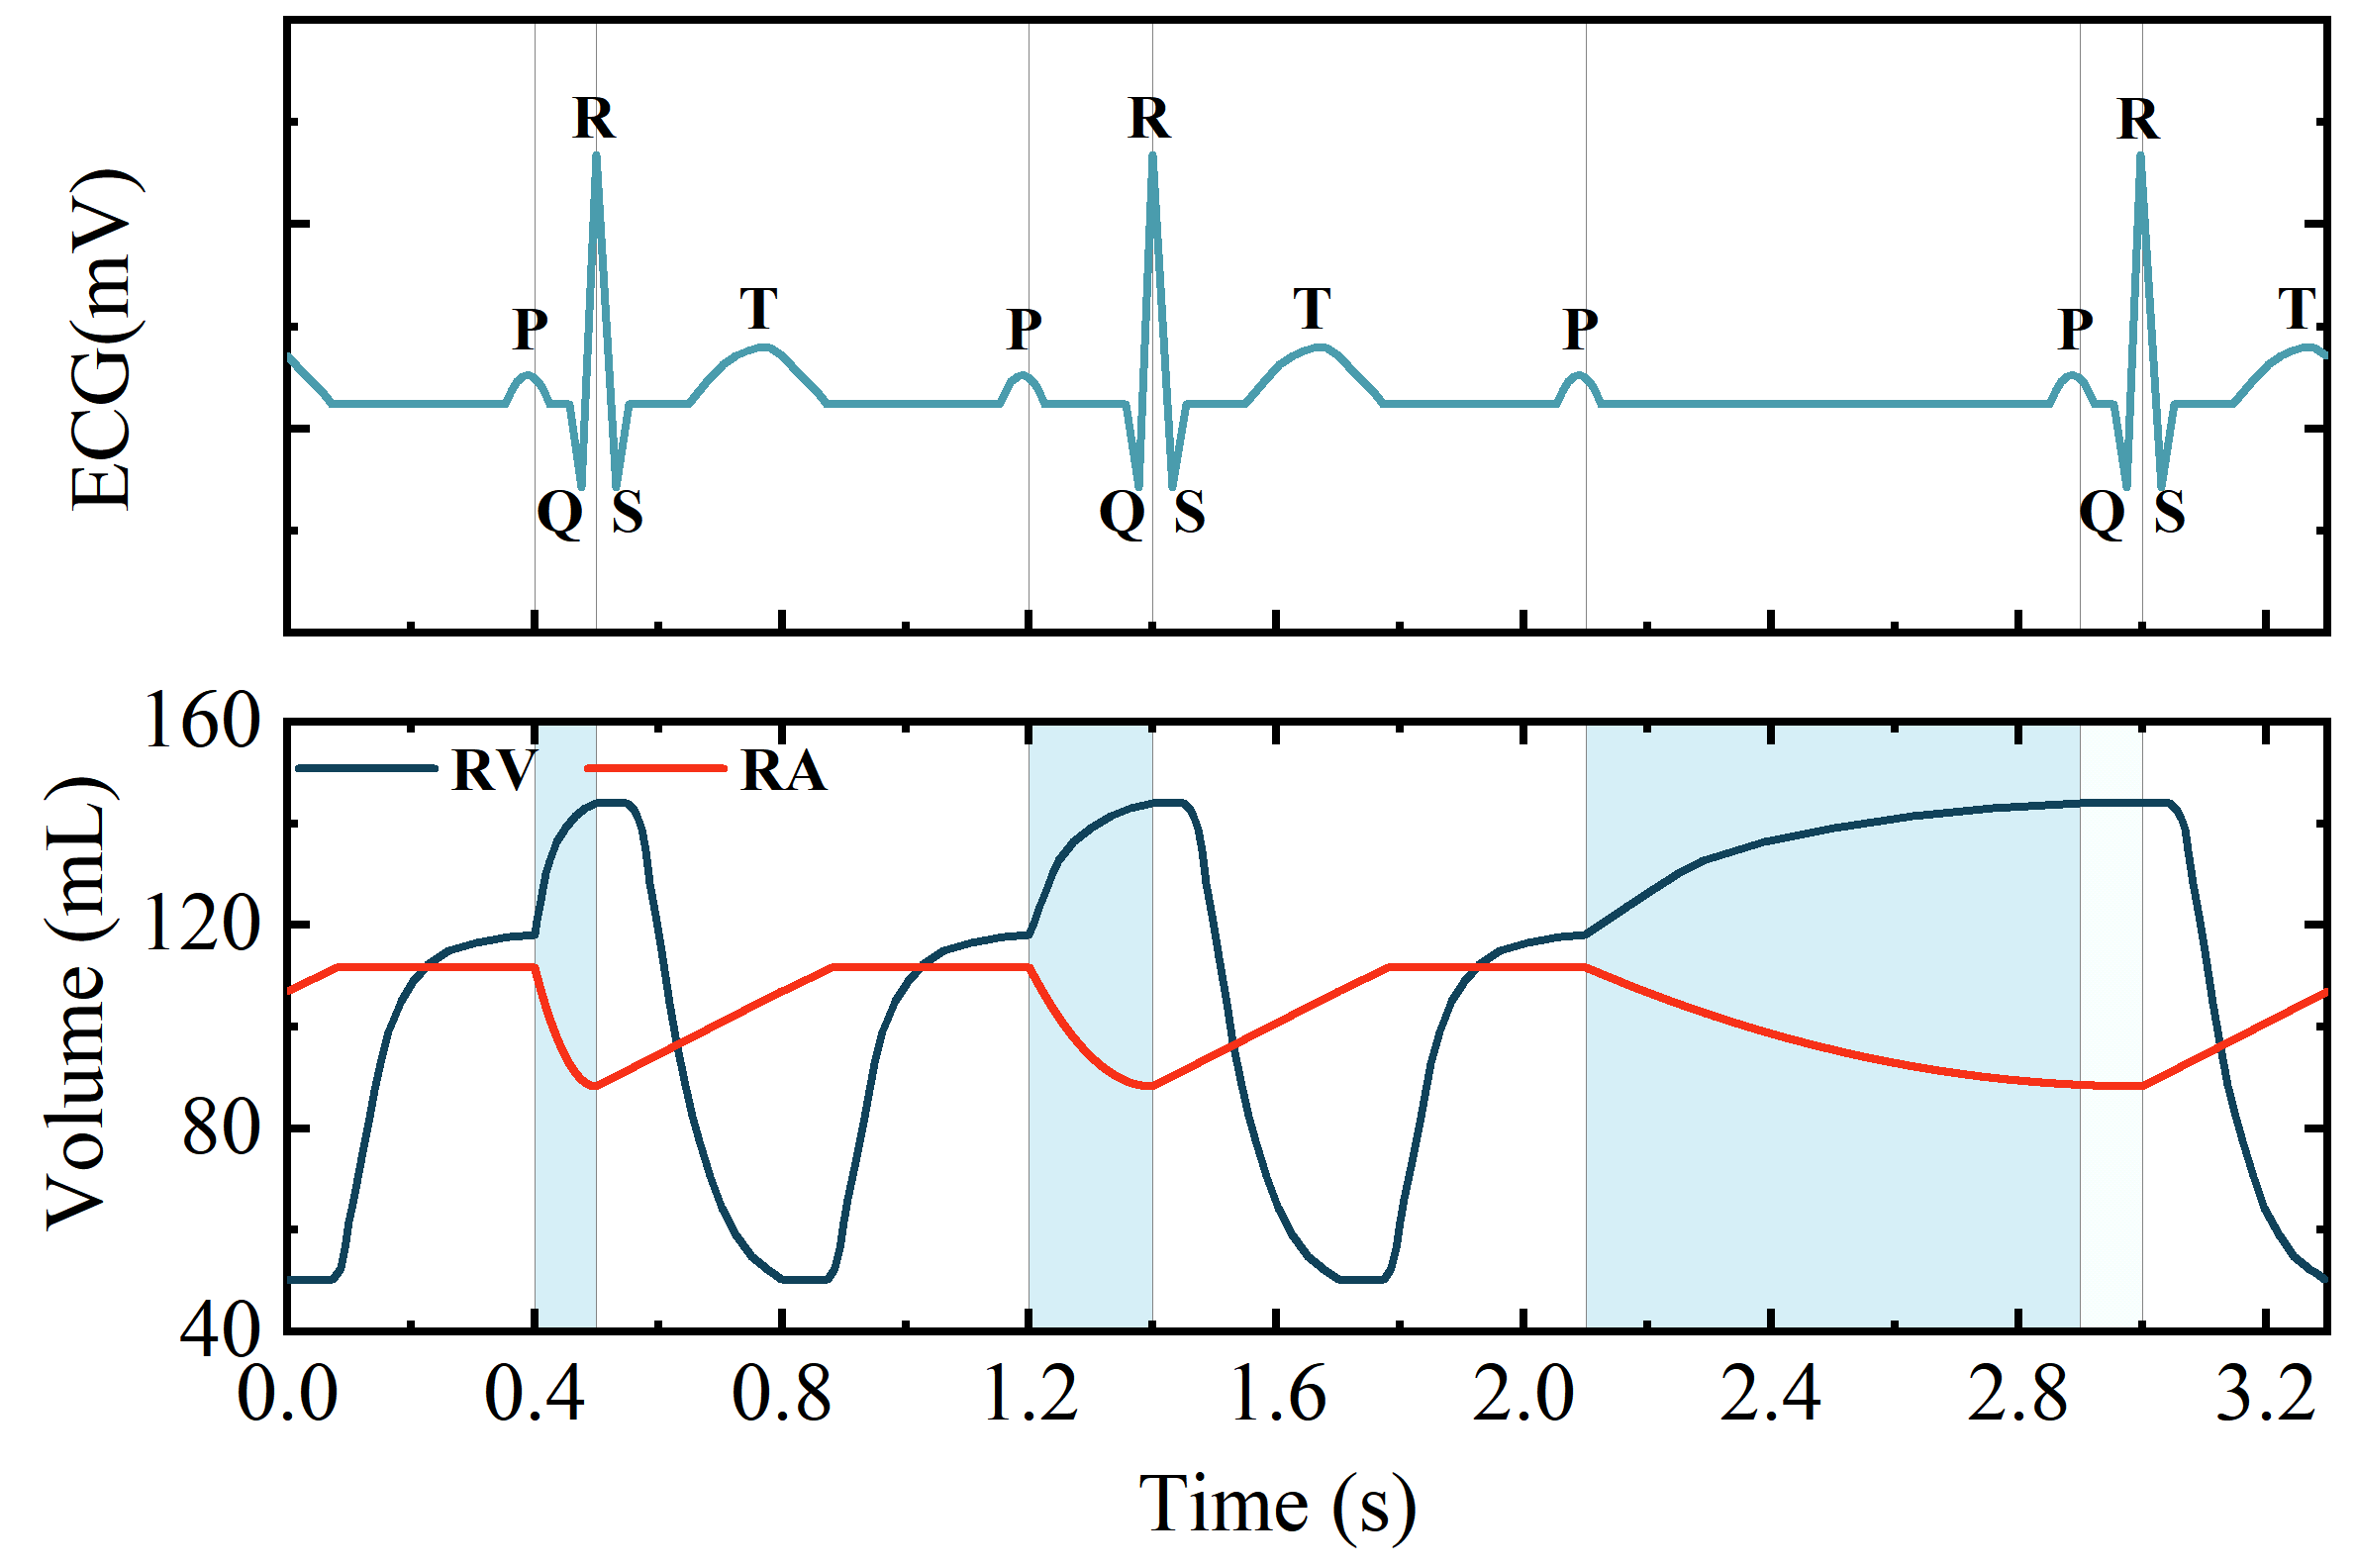
\includegraphics[width=0.9\columnwidth]{Figure/AVB_Vol}
    \caption{Emulation of a pathological cardiac cycle corresponding to our representative AVB model. The mapping illustrates an instance of intermittent conduction failure, where a P-wave is not followed by a QRS complex, leading to an irregular hemodynamic profile.}
    \label{fig:avb_mapping}
\end{figure}

\subsection{Communication System Evaluation Apparatus}
For the end-to-end performance evaluation, the VNA was replaced by the complete transceiver link shown in Fig.~\ref{BER}. The transmitter generated a \SI{1}{\mega\hertz} OOK signal at an average power of \SI{-10}{dBm}, which was coupled into the right atrium. Our custom-developed SRR, integrating the hybrid AGC, was connected to an electrode in the right ventricle. All evaluations were conducted under the emulated representative pathological conditions.

The reliability of the link was quantitatively evaluated by capturing the demodulated binary stream and comparing it offline against the transmitted PRBS to calculate the BER over a data rate range of \SI{500}{bps} to \SI{5}{kbps}. The baseline BER without AGC was also evaluated. To ensure reliability, all procedures were replicated across three independent porcine heart preparations (N=3), with each BER measurement being repeated five times (n=5) and the results averaged.

\begin{figure}[!t]
    \centering
    \includegraphics[width=0.95\columnwidth]{Figure/Mea.BER}
    \caption{Schematic of the experimental setup for BER evaluation. The configuration integrates a signal generator (SG), the \textit{ex-vivo} heart platform, the adaptive SRR, and a data acquisition (DAQ) system.}
    \label{BER}
\end{figure}

\section{Experimental Results}
\label{sec:results}
The performance of the proposed hybrid AGC system was rigorously evaluated. The key findings presented below demonstrate the system's efficacy in mitigating dynamic channel variations, particularly under our simulated representative pathological condition.

\subsection{Dynamic Intracardiac Channel Characteristics}
Fig.~\ref{fig:path_gain_variation} reveals the dynamic nature of the RA-RV intracardiac channel path gain. The results highlight a fundamental difference between ``healthy" and ``pathological" dynamics. Under simulated healthy conditions, as shown in Fig.~\ref{fig:path_gain_variation}(a), the path gain exhibits highly regular, periodic fluctuations that are strictly synchronized with the cardiac cycle. In stark contrast, under the simulated representative pathological conditions of Fig.~\ref{fig:path_gain_variation}(b), the nature of the channel dynamics changes radically. The most critical distinction is the loss of periodicity; due to the ``dropped beats," the channel gain exhibits non-periodic, irregular behavior, making the timing and magnitude of its variations unpredictable. Data from three different heart preparations consistently reproduce this transition from ``regular" to ``irregular," underscoring the profound challenge that such pathological dynamics pose to reliable communication.

\begin{figure}[!t]
    \centering
    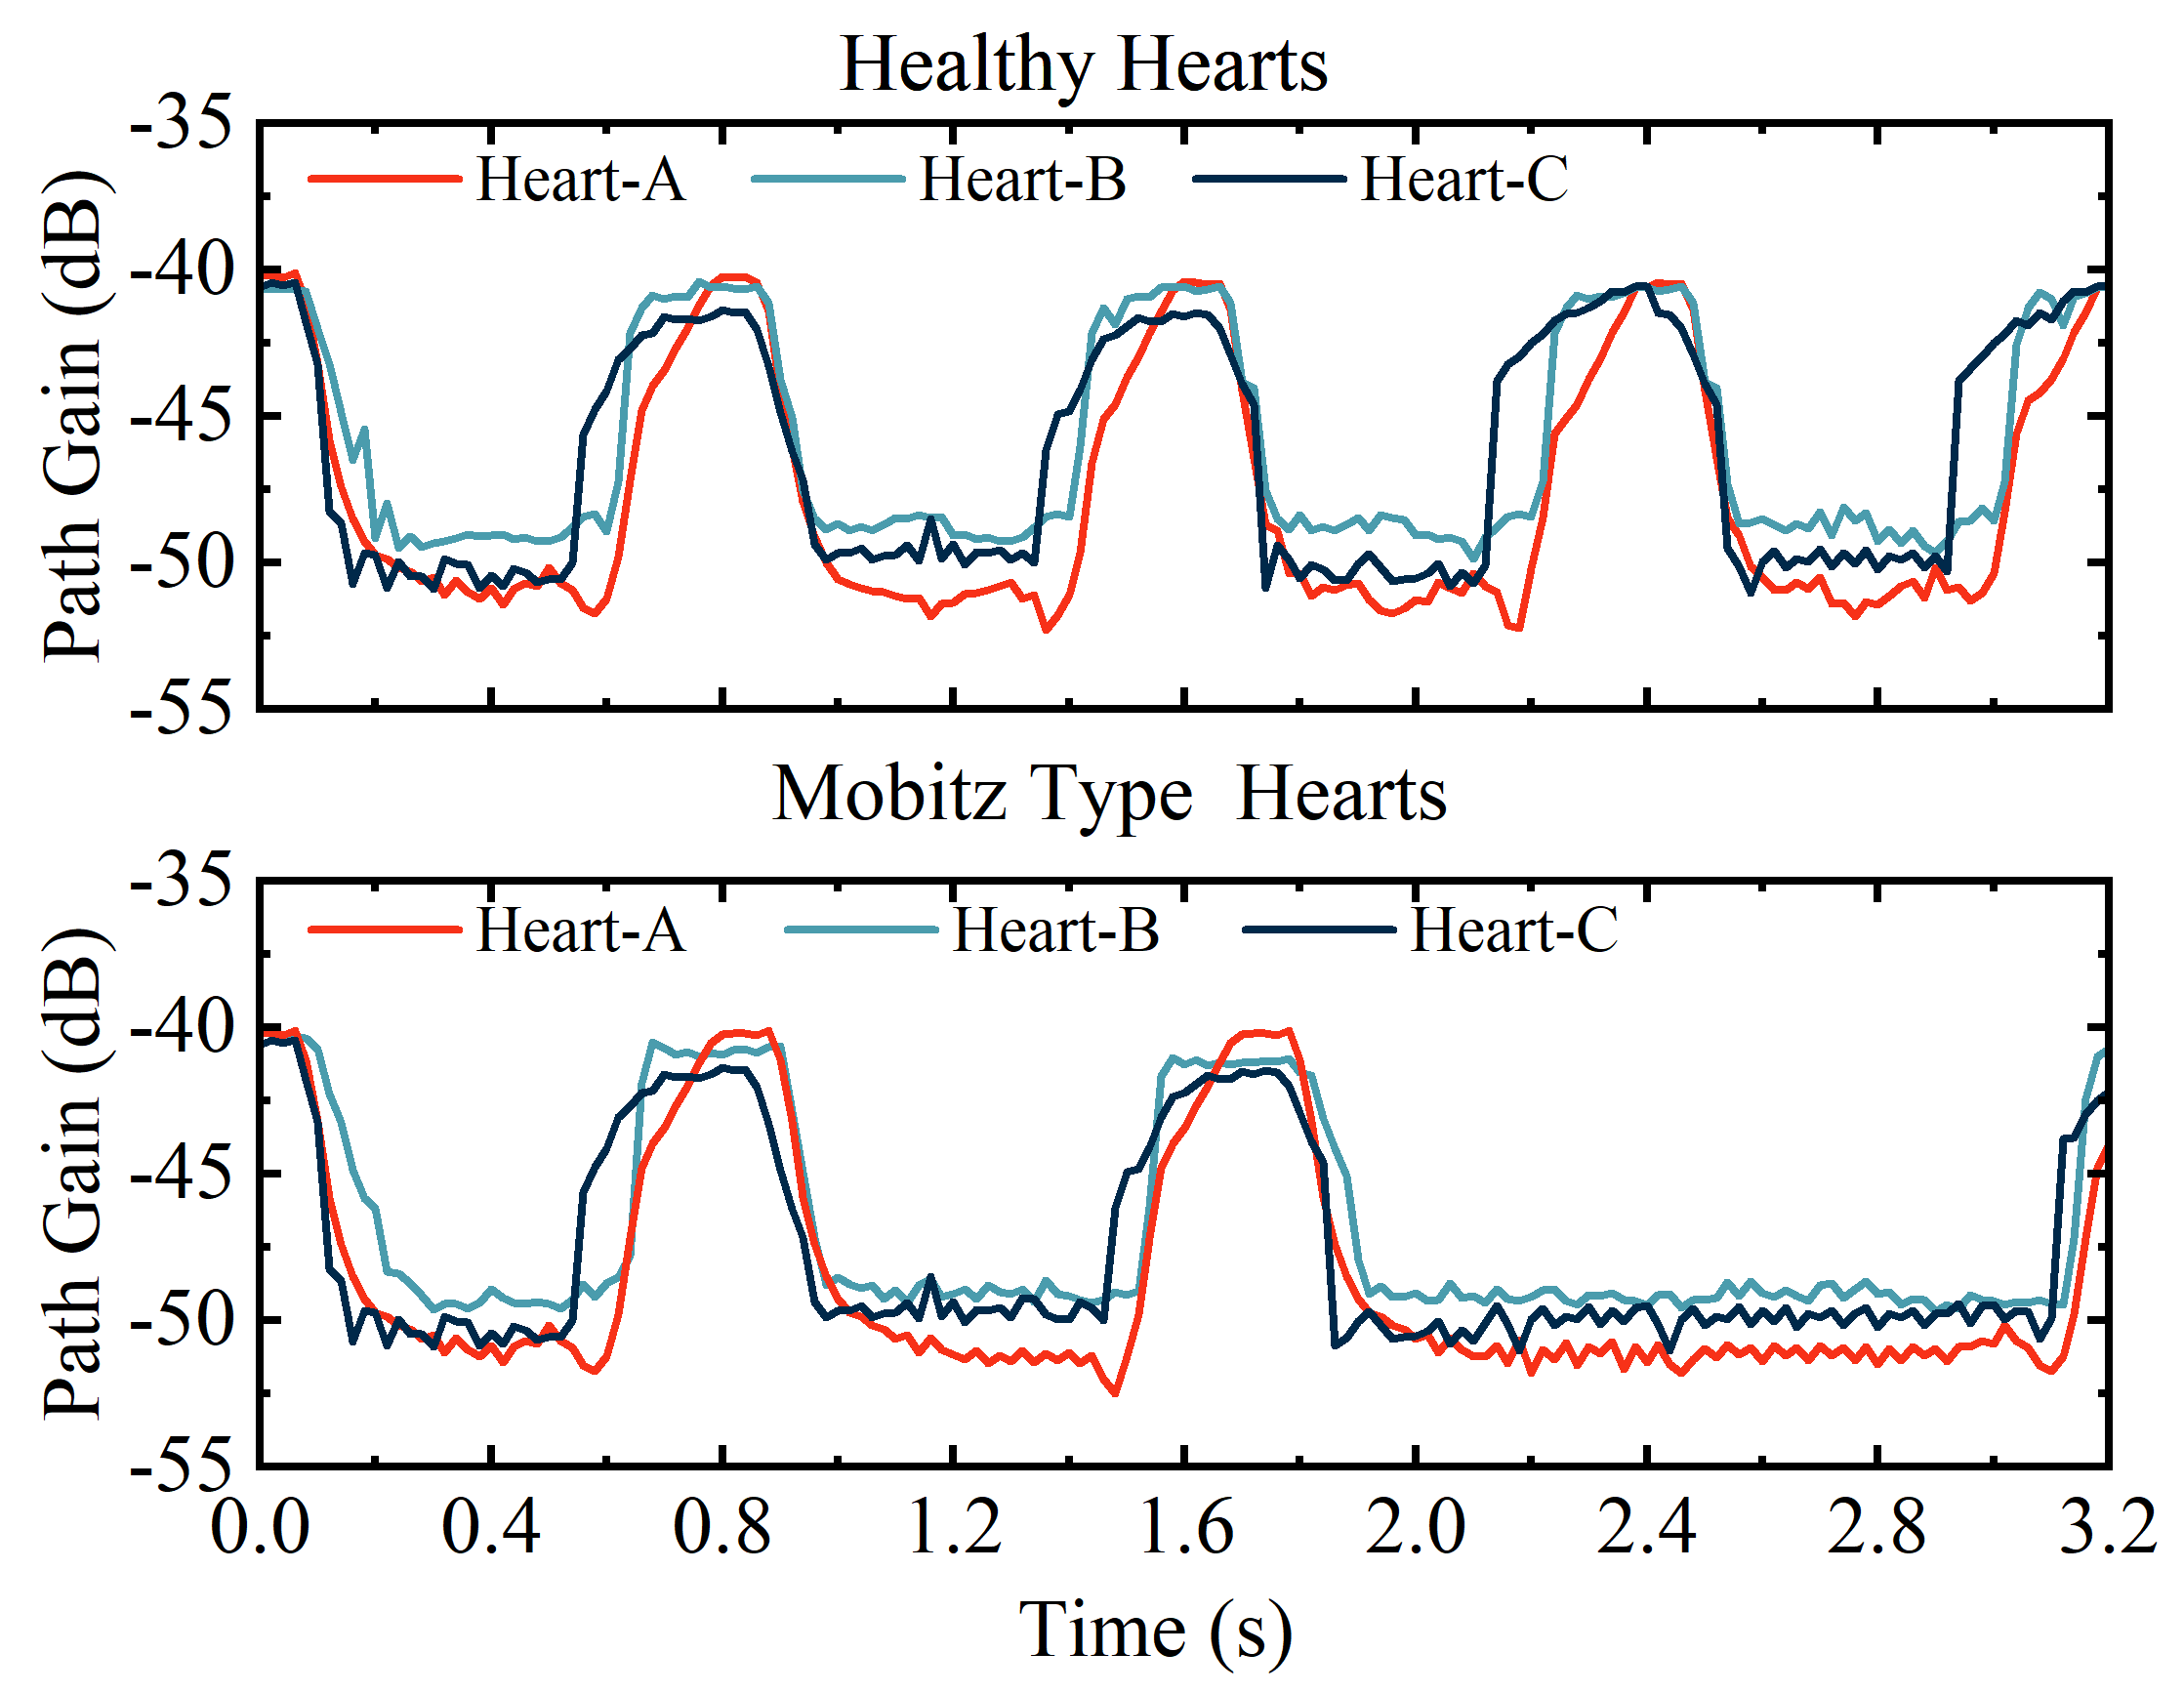
\includegraphics[width=0.9\linewidth]{Figure/signal_heart}
    \caption{Dynamic path gain variation of the RA-RV intracardiac channel. (a) Under simulated healthy heart conditions. (b) Under simulated representative pathological (Mobitz Type I AVB) conditions. Results from three different ex-vivo porcine heart preparations are shown.}
    \label{fig:path_gain_variation}
\end{figure}





\begin{figure}[!t]
    \centering
    \includegraphics[width=9cm]{Figure/STEP}
    \caption{Dynamic path gain variation of the RA-RV intracardiac channel. (a) Under simulated healthy heart conditions. (b) Under simulated representative pathological (Mobitz Type I AVB) conditions. Results from three different ex-vivo porcine heart preparations are shown.}
    \label{fig:step}
\end{figure}

\begin{figure}[!t]
    \centering
    \includegraphics[width=9cm]{Figure/step_all}
    \caption{Dynamic path gain variation of the RA-RV intracardiac channel. (a) Under simulated healthy heart conditions. (b) Under simulated representative pathological (Mobitz Type I AVB) conditions. Results from three different ex-vivo porcine heart preparations are shown.}
    \label{fig:step_all}
\end{figure}

\subsection{AGC System Performance in Signal Stabilization}
The effectiveness of the proposed AGC system in stabilizing the SRR input signal is demonstrated in Figure~\ref{fig:agc_stabilization}. These experiments were conducted under the simulated pathological AVB conditions. The reference ECG signal provides a temporal marker for the cardiac cycle. Without AGC, the received signal amplitude at the SRR input fluctuated significantly from approximately \SI{1.5}{\milli\volt} to \SI{5.0}{\milli\volt}.

In contrast, when the AGC system was activated, the PID controller dynamically adjusted the VGA control voltage ($V_g$). This control voltage exhibited an inverse relationship to the uncompensated signal amplitude, actively modulating the VGA gain to counteract channel fluctuations. Consequently, the SRR input signal amplitude was effectively stabilized around the target level of \SI{100}{\milli\volt}, with residual peak-to-peak fluctuations reduced to less than 1\%. This demonstrates the AGC's capability to provide a consistent signal level to the SRR despite substantial channel dynamics.

\begin{figure}[!t]
    \centering
    \includegraphics[width=0.9\linewidth]{Figure/Receiver_power}
    \caption{Effectiveness of the hybrid AGC system in stabilizing the receiver input signal. (a) Reference ECG signal. (b) Received signal amplitude at the SRR input without AGC. (c) Dynamic VGA control voltage ($V_g$). (d) Stabilized signal amplitude at the SRR input with AGC activated.}
    \label{fig:agc_stabilization}
\end{figure}

\subsection{Impact of AGC on OOK Signal Demodulation}
Figure~\ref{fig:ook_demodulation} provides compelling visual evidence of the proposed AGC's efficacy in enabling robust OOK demodulation. The transmitted baseband sequence is shown in Fig.~\ref{fig:ook_demodulation}(a). After passing through the adaptive front-end, the resulting signal at the SRR input is displayed in Fig.~\ref{fig:ook_demodulation}(b). Critically, even with the underlying dynamic channel, the AGC maintains the amplitude of the OOK bursts at a constant level.

Consequently, the SRR reliably recovers the data, producing the clean baseband output shown in Fig.~\ref{fig:ook_demodulation}(c). The output waveform's timing logic aligns perfectly with the transmitted sequence, and its high-level voltage of approximately 3.3\,V corresponds directly to the supply rail of the output comparator, confirming successful data recovery. This result qualitatively validates that the proposed AGC architecture is essential for preserving signal integrity and ensuring robust communication reliability.

\begin{figure}[!t]
    \centering
    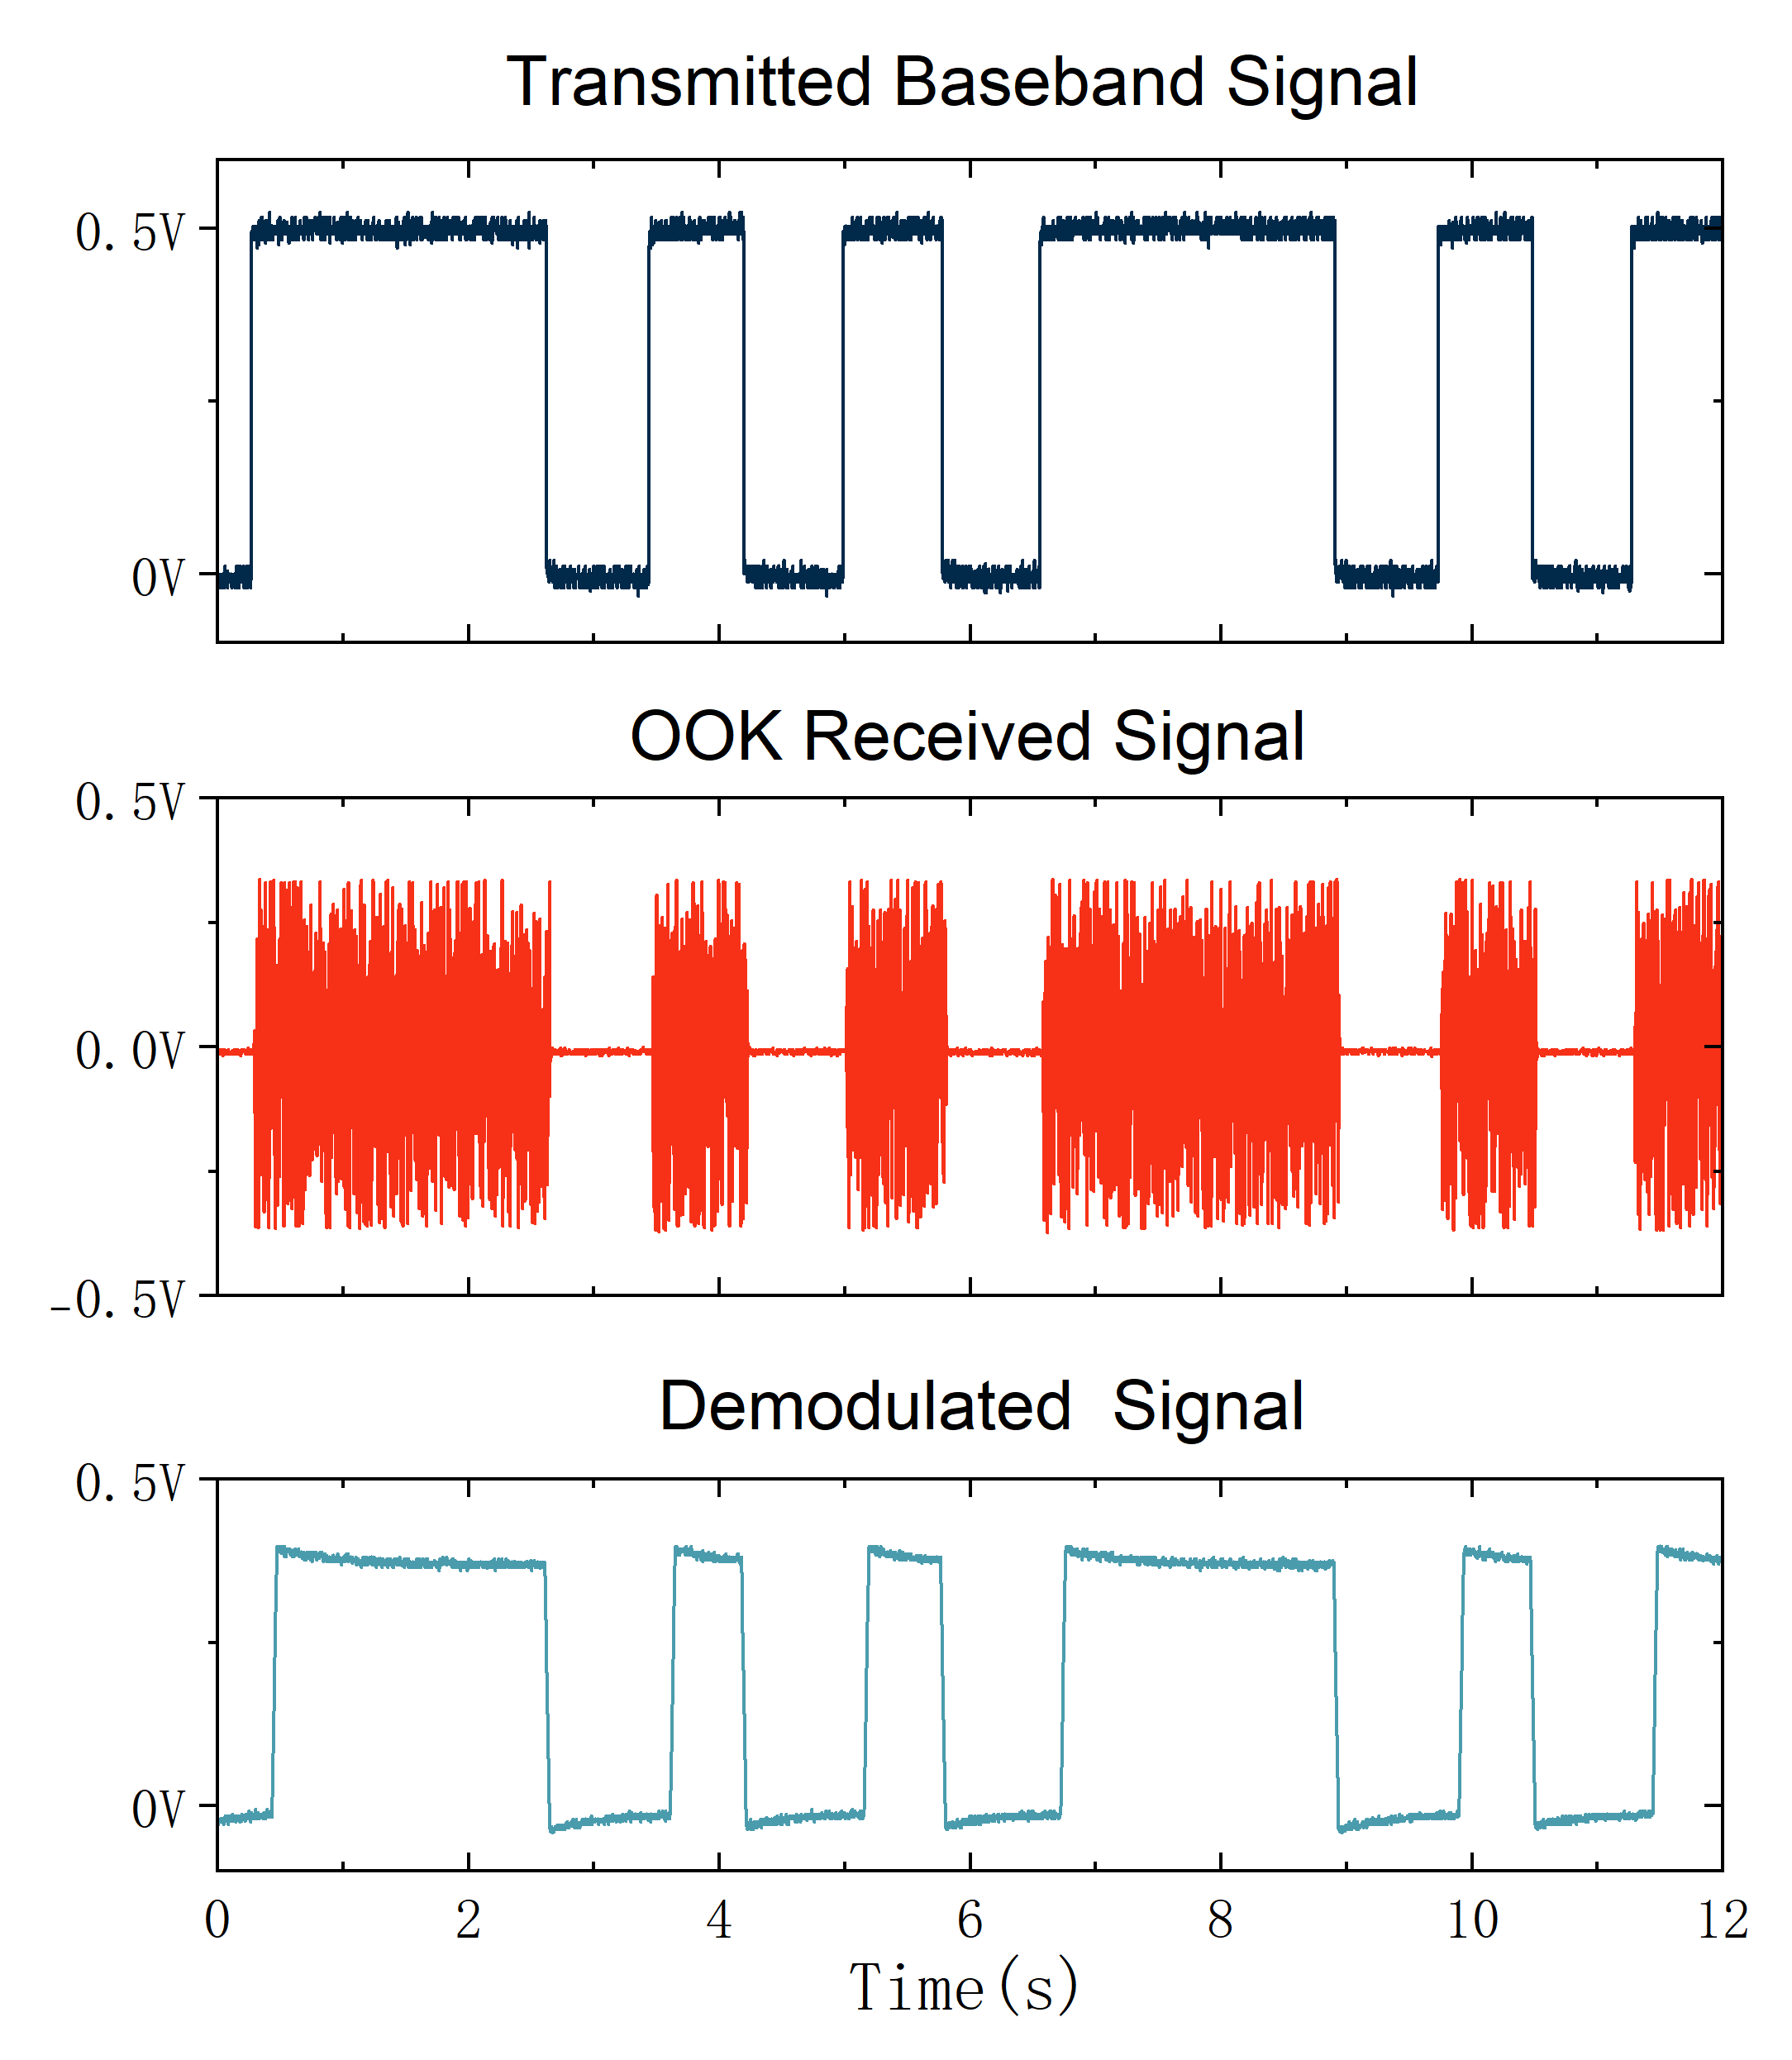
\includegraphics[width=0.8\linewidth]{Figure/ook}
    \caption{OOK signal waveforms at different stages of the system with AGC activated. (a) Transmitted baseband signal. (b) Received signal at the SRR input. (c) Demodulated baseband signal at the SRR output.}
    \label{fig:ook_demodulation}
\end{figure}

\subsection{Bit Error Rate (BER) Improvement}
The ultimate validation of the AGC system's impact on communication reliability was quantified by BER measurements conducted under our representative pathological channel condition. As conclusively demonstrated in Fig.~\ref{fig:ber_performance}, the proposed AGC architecture offers a profound advantage. Throughout the entire operational range (\SI{500}{bps} to \SI{5}{kbps}), activating the AGC reduces the BER by more than an order of magnitude compared to the non-AGC case. At \SI{3}{kbps}, for example, the BER improves from \num{4.5e-4} to \num{9e-5}, transforming the link's reliability from intermittent to highly robust.

Even more revealing is the trend highlighted by the percentage improvement, which systematically climbs from 54.8\% at \SI{500}{bps} to an impressive 83.7\% at \SI{5}{kbps}. This trend offers a critical insight: higher data rates, with their shorter symbol durations, are inherently less tolerant of signal amplitude instability. Consequently, the signal stabilization provided by the AGC becomes increasingly beneficial—yielding a greater performance ``dividend"—as the communication speed increases.

Finally, the minimal error bars, representing the standard deviation across three independent heart preparations (N=3), offer powerful statistical validation of the method's robustness. They confirm that the substantial performance gains are not sample-specific but are highly repeatable and generalizable, which is paramount for any potential clinical translation.

\begin{figure}[!t]
    \centering
    \includegraphics[width=0.8\linewidth]{Figure/BER}
    \caption{BER performance comparison with and without AGC across different data rates under the simulated representative pathological condition. The yellow line indicates the percentage improvement in BER. Error bars represent the standard deviation across N=3 independent heart preparations.}
    \label{fig:ber_performance}
\end{figure}

\begin{table*}[htbp]
\centering
\caption{PERFORMANCE COMPARISON WITH RELATED RECEIVER PROTOTYPES}
\label{tab:comparison_modified}
\begin{tabularx}{\textwidth}{l >{\raggedright\arraybackslash}X >{\raggedright\arraybackslash}X >{\raggedright\arraybackslash}X >{\raggedright\arraybackslash}X >{\raggedright\arraybackslash}X}
\toprule
\bfseries Metric & \bfseries Bereuter et al.~\cite{bereuter2019leadless} & \bfseries Ryser et al.~\cite{ryser2022modulation} & \bfseries Khaleghi et al.~\cite{khaleghi2020conductive} & \bfseries Yuk et al.~\cite{yuk2020implantable} & \bfseries This Work \\
\midrule
\textbf{Core Contribution} & In-vivo Channel Characterization & Modulation Scheme Analysis & Wideband Channel Modeling & Low-Power IC & \textbf{Pathological Channel Robustness} \\
\addlinespace
\bfseries Measurement Type & In-vivo & In-vitro & In-vitro & In-vivo / In-vitro & In-vitro (Simulated Pathology) \\
\addlinespace
\bfseries Frequency [MHz] & 1 & 1.5 & 0.01-10 & DC-20 & 1 \\
\addlinespace
\bfseries RX Power [mW] & >465 & 152 & 230 & \textbf{0.062} & 268 \\
\addlinespace
\bfseries Technology & Discrete & Discrete & Discrete & \textbf{110nm CMOS} & Discrete (Proof-of-Concept) \\
\bottomrule
\end{tabularx}
\end{table*}

\section{Discussion}
\label{sec:discussion}
The experimental results of this study not only validate the effectiveness of our proposed hybrid AGC-SRR architecture but, more importantly, offer profound insights into countering the harsh intracardiac communication environment induced by pathological rhythms. Our core finding—a BER improvement of up to 83.7\%—transcends a mere numerical result. It experimentally quantifies for the first time the devastating impact of a ``pathological channel" on communication reliability and demonstrates that active, real-time gain compensation is a fundamental strategy for ensuring the reliability of LCPs in clinical scenarios. The most critical insight from this work is that the design paradigm for these systems must shift from adapting to the predictable, periodic fluctuations of a healthy heart to tracking the unpredictable, chaotic fluctuations of a pathological one.

The success of our proposed architecture in tackling this challenge stems from its inherent design rationale. The waveforms in Fig.~\ref{fig:agc_stabilization} show that the VGA control voltage exhibits a clear inverse correlation with the uncompensated signal fluctuations, indicating that the analog front-end can rapidly track channel transients caused by events such as dropped beats. Concurrently, the stabilized signal, with its residual fluctuations suppressed to within 1\%, proves that the digital PID controller achieves high-precision steady-state control. It is this combination of rapid tracking and precise steady-state control that enables the system to effectively combat aperiodic, severe fluctuations.

Placing this research within its evolutionary context highlights its pioneering nature. Early research stages focused on characterizing the channel under static conditions. Subsequently, research entered a second phase, exploring ``healthy dynamics," such as our team's prior modeling work~\cite{wei2024time}. The core contribution of this paper is to advance the research into a third, and most clinically challenging, stage: ``pathological dynamics." We are the first to systematically shift the focus to the irregular channel environment induced by a real-world pathology and to propose a validated adaptive receiver architecture designed to conquer such a harsh channel. This critical leap from ``healthy" to ``pathological" dynamics represents a decisive step toward clinically robust applications.

We must also critically examine the boundaries of this study. Our \textit{ex-vivo} platform, while enabling the precise reproduction of dynamics induced by our chosen representative pathology, cannot fully replicate all complexities of a true in-vivo environment, such as autonomic nervous system regulation and long-term tissue-electrode interface responses. Furthermore, our current system is a proof-of-concept prototype built from discrete components. Its value lies not in providing an immediately implantable device but in offering a rigorously validated design blueprint for future ASIC development. The use of discrete components provided the necessary flexibility for rapid iteration and validation of the core control algorithm.

Based on this analysis, the path for future research is clear. Technologically, the primary task is the full-custom CMOS implementation of the validated architecture to reduce power and size. Scientifically, it is necessary to advance our validation methodology from ex-vivo models to long-term in-vivo studies in large animal models. This will allow for the assessment of long-term stability and enable the investigation of a wider range of pathological models, ultimately propelling this technology toward clinical translation.
%
%本研究的实验结果不仅验证了我们提出的混合AGC-SRR架构的有效性，更重要的是，为应对由病理性节律引发的恶劣心内通信环境提供了深刻见解。我们的核心发现——误码率（BER）改善高达83.7%——不仅仅是一个数字结果。它首次通过实验量化了“病理性信道”对通信可靠性的破坏性影响，并证明主动、实时的增益补偿是确保临床场景下心腔内通信设备（LCPs）可靠性的基本策略。这项工作最关键的见解是，这些系统的设计范式必须从适应健康心脏可预测的、周期性的波动，转变为跟踪病理性心脏不可预测的、混沌的波动。
%
%我们提出的架构之所以能成功应对这一挑战，源于其内在的设计理念。图\ref{fig:agc_stabilization}中的波形显示，可变增益放大器（VGA）的控制电压与未补偿的信号波动呈现明显的反相关关系，这表明模拟前端能够快速跟踪由漏搏等事件引起的信道瞬变。同时，经稳定后的信号其残余波动被抑制在1%以内，这证明数字比例-积分-微分（PID）控制器实现了高精度的稳态控制。正是这种快速跟踪与精确稳态控制的结合，使系统能够有效对抗非周期性的剧烈波动。
%
%将本研究置于其发展背景中，更能凸显其开创性。早期研究阶段侧重于静的信道特性分析。随后，研究进入第二阶段，探索“健康动态”，例如我们团队先前的建模工作\cite{wei2024time}。本文的核心贡献在于将研究推进到第三个阶段，也是临床上面临最大挑战的阶段：“病理性动态”。我们首次系统性地将研究重点转向由真实病理状态引发的不规则信道环境，并提出了一种经过验证的自适应接收器架构，旨在攻克这种恶劣的信道条件。这种从“健康”到“病理性”动态的关键跨越，代表着向临床稳健应用迈出的决定性一步。
%
%我们还必须审慎审视本研究的局限性。我们的体外（ex-vivo）平台虽然能够精确复现我们所选代表性病理引发的动态变化，但无法完全复制真实体内（in-vivo）环境的所有复杂性，例如自主神经系统调节以及长期的组织-电极界面反应。此外，我们当前的系统是一个由分立元件构建的概念验证原型。其价值不在于提供一种可立即植入的设备，而在于为未来的专用集成电路（ASIC）开发提供经过严格验证的设计蓝图。分立元件的使用为核心控制算法的快速迭代和验证提供了必要的灵活性。
%
%基于上述分析，未来的研究方向清晰可见。在技术层面，主要任务是对已验证的架构进行全定制互补金属氧化物半导体（CMOS）实现，以降低功耗和尺寸。在科学层面，有必要将我们的验证方法从体外模型推进到大型动物模型的长期体内研究。这将有助于评估长期稳定性，并能研究更广泛的病理模型，最终推动这项技术向临床转化。

\section{Conclusion}
\label{sec:conclusion}

This paper confronted the core challenge of achieving robust communication for networked IMDs within dynamic, pathological biological environments. Using multi-chamber leadless pacemakers as a test case, we proposed and successfully validated a novel adaptive receiver architecture designed to conquer the severe and irregular channel fluctuations induced by pathological cardiac rhythms characterized by intermittent conduction failure.

Through rigorous testing on an \textit{ex-vivo} cardiac platform that we developed to precisely emulate a representative pathological dynamic, the architecture demonstrated exceptional performance. The results provide definitive proof that the proposed AGC system can stabilize the received signal to within 1\% of its target value amidst channel gain fluctuations exceeding 15\,dB, ultimately achieving a BER improvement of up to 83.7\%.

In conclusion, this research not only provides a key enabling technology for clinically reliable multi-chamber LCPs but, more importantly, offers a rigorously validated and universally applicable design paradigm for the next generation of networked IMDs intended to operate robustly in harsh biological environments. Future work will focus on the CMOS integrated circuit implementation of this architecture to accelerate its translation to eventual clinical use.

\bibliographystyle{ieeetr}
\bibliography{Reference}

\end{document}